\subsection{HAUSDORFF SPACES}

PROPOSITION 1. Let X be a topological space. Then the following statements are equivalent:

\begin{enumerate}
\def\labelenumi{(\Alph{enumi})}
\setcounter{enumi}{7}
\tightlist
\item
  Any two distinct points of X have disjoint neighbourhoods.
\end{enumerate}

(Hi) The intersection of the closed neighbourhoods of any point of X consists of that point alone.

(Hii) The diagonal of the product space \(\mathbf{X} \times \mathbf{X}\) is a closed set.

(Hiii) For every set I, the diagonal of the product space Y = X \(^{I}\) is closed in Y.

\((\mathbf{H}^{\mathrm{iv}})\) No filter on \(\mathbf{X}\) has more than one limit point.

(Hv) If a filter \(\mathfrak{F}\) on X converges to \(x\) , then \(x\) is the only cluster point of \(\mathfrak{F}\) .

We shall prove the implications

and

\[
\begin{array}{r l} (\mathrm{H}) & \Longrightarrow (\mathrm{H} ^ {\mathrm{i}}) \Longrightarrow (\mathrm{H} ^ {\mathrm{v}}) \Longrightarrow (\mathrm{H} ^ {\mathrm{iv}}) \Longrightarrow (\mathrm{H}) \\ (\mathrm{H}) & \Longrightarrow (\mathrm{H} ^ {\mathrm{iii}}) \Longrightarrow (\mathrm{H} ^ {\mathrm{ii}}) \Longrightarrow (\mathrm{H}). \end{array}
\]

\((\mathrm{H}) \Longrightarrow (\mathrm{H}^{\mathrm{i}}): \text{ If } x \neq y \text{ there is an open neighbourhood } \mathrm{U} \text{ of } x \text{ and an open neighbourhood } \mathrm{V} \text{ of } y \text{ such that } \mathrm{U} \cap \mathrm{V} = \varnothing; \text{ hence } y \notin \overline{\mathrm{U}}.\)

\((\mathbf{H}^{\mathrm{i}}) \Longrightarrow (\mathbf{H}^{\mathrm{v}}): \text{ Let } y \neq x; \text{ then there is a closed neighbourhood } V \text{ of } x \text{ such that } y \notin V, \text{ and by hypothesis there exists } M \in \mathfrak{F} \text{ such that } M \subset V; \text{ thus } M \cap \mathbb{C}V = \emptyset. \text{ But } \mathbb{C}V \text{ is a neighbourhood of } y; \text{ hence } y \text{ is not a cluster point of } \mathfrak{F}.\)

\((\mathbf{H}^{\mathrm{v}}) \Rightarrow (\mathbf{H}^{\mathrm{iv}})\) : Clear, since every limit point of a filter is also a cluster point.

\((\mathrm{H}^{\mathrm{iv}}) \Longrightarrow (\mathrm{H})\) : Suppose \(x \neq y\) and that every neighbourhood \(V\) of \(x\) meets every neighbourhood \(W\) of \(y\) . Then the sets \(V \cap W\) form a base of a filter which has both \(x\) and \(y\) as limit points, which is contrary to hypothesis.

\((\mathrm{H}) \Longrightarrow (\mathrm{H}^{\mathrm{iii}})\) : Let \((x) = (x_{\iota})\) be a point of \(\mathbf{X}^{\mathbf{I}}\) which does not belong to the diagonal \(\Delta\) . Then there are at least two indices \(\lambda, \mu\) such that \(x_{\lambda} \neq x_{\mu}\) . Let \(\mathbf{V}_{\lambda}\) (resp. \(\mathbf{V}_{\mu}\) ) be a neighbourhood of \(x_{\lambda}\) (resp. \(x_{\mu}\) ) in \(\mathbf{X}\) , such that \(\mathbf{V}_{\lambda} \cap \mathbf{V}_{\mu} = \emptyset\) ; then the set \(W = V_{\lambda} \times V_{\mu} \times \prod_{\iota \neq \lambda, \mu} X_{\iota}\) (where \(X_{\iota} = X\) if \(\iota \neq \lambda, \mu\) ) is a neighbourhood of \(x\) in \(X^{\mathbf{I}}\) ( \(\S 4, no.1\) ) which does not meet \(\Delta\) . Hence \(\Delta\) is closed in \(X^{\mathbf{I}}\) .

\((\mathbf{H}^{\mathrm{iii}}) \Rightarrow (\mathbf{H}^{\mathrm{ii}}): \text{Obvious.}\)

\((H^{ii}) \Longrightarrow (H)\) : If \(x \neq y\) then \((x, y) \in X \times X\) is not in the diagonal \(\Delta\) , hence (§ 4, no. 1) there is a neighbourhood \(V\) of \(x\) and a neighbourhood \(W\) of \(y\) in \(X\) such that \((V \times W) \cap \Delta = \emptyset\) , which means that

\[
\mathbf {V} \cap \mathbf {W} = \varnothing .
\]

DEFINITION 1. A topological space satisfying the conditions of Proposition 1 is called a Hausdorff or separated space; the topology of such a space is said to be a Hausdorff topology.

Axiom (H) is Hausdorff's axiom.

Examples. Any discrete space is Hausdorff. The rational line Q is Hausdorff, for if x, y are two rational numbers such that x \textless{} y then there is a rational number z such that x \textless{} z \textless{} y, and the neighbourhoods {]}\(\leftarrow\) , z{[} of x and {]}z, \(\rightarrow\) {[} of y do not intersect.

A set X having at least two points and carrying the coarsest topology (§ 2, no. 2) is not a Hausdorff space.

Let \(f: X \to Y\) be a mapping of a set \(X\) into a Hausdorff space \(Y\) ; then it follows immediately from Proposition 1 that \(f\) can have at most one limit with respect to a filter \(\mathfrak{F}\) on \(X\) , and that if \(f\) has \(y\) as a limit with respect to \(\mathfrak{F}\) , then \(y\) is the only cluster point of \(f\) with respect to \(\mathfrak{F}\) .

PROPOSITION 2. Let \(f, g\) be two continuous mappings of a topological space \(\mathbf{X}\) into a Hausdorff space \(\mathbf{Y}\) ; then the set of all \(x \in \mathbf{X}\) such that \(f(x) = g(x)\) is closed in \(\mathbf{X}\) .

For this set is the inverse image of the diagonal of \(\mathbf{Y} \times \mathbf{Y}\) under the mapping \(x \to (f(x), g(x))\) , which is continuous ( \(\S 4\) , no. 1, Proposition 1). The result therefore follows from (H \(^{ii}\) ) and \(\S 2\) , no. 1, Theorem 1.

COROLLARY I (Principle of extension of identities). Let \(f, g\) be two continuous mappings of a topological space \(X\) into a Hausdorff space \(Y\) . If \(f(x) = g(x)\) at all points of a dense subset of \(X\) , then \(f = g\) .

In other words, a continuous map of X into Y (Hausdorff) is uniquely determined by its values at all points of a dense subset of X.

COROLLARY 2. If \(f\) is a continuous mapping of a topological space \(\mathbf{X}\) into a Hausdorff space \(\mathbf{Y}\) , then the graph of \(f\) is closed in \(\mathbf{X} \times \mathbf{Y}\) .

For this graph is the set of all \((x, y) \in \mathbf{X} \times \mathbf{Y}\) such that \(f(x) = y\) , and the two mappings \((x, y) \to y\) and \((x, y) \to f(x)\) are continuous.

PROPOSITION 3. Let \((x_{i})_{1\leqslant i\leqslant n}\) be a finite family of distinct points of a Hausdorff space \(\mathbf{X}\) ; then each \(x_{i}\) has a neighbourhood \(\mathbf{V}_{i}\) in \(\mathbf{X}\) such that the \(\mathbf{V}_{i}\) ( \(1\leqslant i\leqslant n\) ) are mutually disjoint.

The proof is by induction on \(n\) : the case \(n = 2\) is just the axiom (H). Let then \(W_i\) ( \(1 \leqslant i \leqslant n - 1\) ) be a neighbourhood of \(x_i\) such that the \(W_i\) are mutually disjoint. On the other hand, for \(1 \leqslant i \leqslant n - 1\) there is a neighbourhood \(T_i\) of \(x_i\) and a neighbourhood \(U_i\) of \(x_n\) which do not intersect. If we take \(V_i\) to be \(W_i \cap T_i\) for \(1 \leqslant i \leqslant n - 1\) and

\[
\mathrm{V} _ {n} = \bigcap_ {i = 1} ^ {n - 1} \mathrm{U} _ {i},
\]

the conditions of the proposition are satisfied.

COROLLARY. Every finite Hausdorff space is discrete.

PROPOSITION 4. Every finite subset of a Hausdorff space is closed.

For every subset consisting of a single point is closed by reason of axiom (H \(^{i}\) ).

PROPOSITION 5. Let X be a topological space and suppose that for each pair of distinct points x, y of X there is a continuous mapping f of X into a Hausdorff space \(X'\) such that \(f(x) \neq f(y)\) . Then X is Hausdorff.

Let \(V'\) and \(W'\) be disjoint neighbourhoods of \(f(x)\) and \(f(y)\) respectively in \(X'\) ; then \(\overline{f}^1(V')\) and \(\overline{f}^1(W')\) are disjoint neighbourhoods of \(x\) and \(y\) respectively in \(X\) .

COROLLARY. Every topology which is finer than a Hausdorff topology is Hausdorff.

\subsection{SUBSPACES AND PRODUCTS OF HAUSDORFF SPACES}

A subspace A of a Hausdorff space X is Hausdorff, as we see by applying Proposition 5 of no. 1 to the canonical injection A → X. Conversely, we have

PROPOSITION 6. If every point of a topological space X has a closed neighbourhood which is a Hausdorff subspace of X, then X is Hausdorff.

Let \(x \in X\) and let \(V\) be a closed neighbourhood of \(x\) in \(X\) such that the subspace \(V\) is Hausdorff. Then the closed neighbourhoods of \(x\) in \(V\) have \(\{x\}\) as their intersection (axiom \((H^i)\) ); but they are also closed neighbourhoods of \(x\) in \(X\) ( \(\S 3, no. 1\) ) and therefore \(X\) satisfies \((H^i)\) .

\pandocbounded{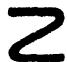
\includegraphics[keepaspectratio]{images/part001_a9a6e172.jpg}}

There exist non-Hausdorff spaces in which every point has a Hausdorff neighbourhood (Exercise 7).

PROPOSITION 7. Every product of Hausdorff spaces is Hausdorff. Conversely, if a product of non-empty spaces is Hausdorff, then each factor is a Hausdorff space.

Let \(X = \prod_{i \in I} X_i\) be a product of topological spaces. Then if \(x, y\) are two distinct points of \(X\) , we have \(\text{pr}_i x \neq \text{pr}_i y\) for some index \(i\) , and Proposition 5 of no. 1 shows that \(X\) is Hausdorff if the \(X_i\) are. Conversely, if \(X\) is Hausdorff and the \(X_i\) are non-empty, then each \(X_i\) is homeomorphic to a subspace of \(X\) ( \(\S 4\) , no. 2, Proposition 4) and is therefore Hausdorff.

COROLLARY I. Let X be a set, let \((\mathbf{Y}_{\iota})_{\iota \in \mathbf{I}}\) be a family of Hausdorff topological spaces, and for each \(\iota \in I\) let \(f_{\iota}\) be a mapping of X into \(Y_{\iota}\) . Let X carry the coarsest topology \(\mathfrak{T}\) for which the \(f_{\iota}\) are continuous. Then a necessary and sufficient condition for X to be Hausdorff is that for each pair of distinct points x, y of X we have \(f_{\iota}(x) \neq f_{\iota}(y)\) for some index \(\iota \in I\) .

The condition is sufficient by reason of Proposition 5 of no. 1. Conversely, suppose X is Hausdorff; let \(Y = \prod_{\iota \in I} Y_{\iota}\) and let \(f = (f_{\iota})_{\iota \in I}\) be the mapping \(x \to (f_{\iota}(x))\) . By Proposition 7 above Y is Hausdorff, and by Proposition 3 of §4, no. 1, \(\mathfrak{T}\) is the inverse image under f of the topology of Y. If \(f(x) = f(y)\) for two distinct points x, y of X it is clear that every open set (in the topology \(\mathfrak{T}\)) which contains x also contains y, contrary to the hypothesis that X is Hausdorff.

COROLLARY 2. Let \((\mathbf{X}_{\alpha}, f_{\alpha \beta})\) be an inverse system of topological spaces. If the \(\mathbf{X}_{\alpha}\) are Hausdorff, then \(\mathbf{X} = \varprojlim \mathbf{X}_{\alpha}\) is Hausdorff and is a closed subspace of \(\prod_{\alpha} \mathbf{X}_{\alpha}\) .

The first assertion follows from the fact that X is a subspace of the Hausdorff space \(\prod_{\alpha} X_{\alpha}\) (Proposition 7). To show that X is closed in the product space, let \(F_{\alpha\beta} (\alpha \leqslant \beta)\) be the subset of \(\prod_{\alpha} X_{\alpha}\) consisting of points x for which \(\operatorname{pr}_{\alpha}x = f_{\alpha\beta}(\operatorname{pr}_{\beta}x)\) ; the \(F_{\alpha\beta}\) are closed in \(\prod_{\alpha} X_{\alpha}\) (no. 1, Proposition 2), hence so is their intersection X.

Evidently, any sum of Hausdorff spaces (§ 2, no. 4, Example 3) is a Hausdorff space.

\subsection{HAUSDORFF QUOTIENT SPACES}

Let us look for conditions under which a quotient space X/R is Hausdorff (in which case the equivalence relation R is said to be Hausdorff). In the first place, if X/R is Hausdorff, then the subsets of X/R consisting of a single point are closed (no. 1, Proposition 4) and hence each equivalence class mod R is closed in X. But this necessary condition is not sufficient.

The definition of open sets in X/R gives rise to the following necessary and sufficient condition: X/R is Hausdorff if and only if any two distinct equivalence classes in X are contained in disjoint saturated open subsets of X. We shall give other more usable conditions.

PROPOSITION 8. A necessary condition for the quotient space X/R to be Hausdorff is that the graph C of R is closed in X × X. If the equivalence relation R is open, this condition is also sufficient.

Let \(\varphi: X \to X/R\) be the canonical mapping; then \(C\) is the inverse image under \(\varphi \times \varphi: X \times X \to (X/R) \times (X/R)\) of the diagonal \(\Delta\) of \((X/R) \times (X/R)\) . The first part of the proposition therefore follows from the continuity of \(\varphi \times \varphi\) {[}Axiom \((H^{ii})\) and Theorem 1 of §2, no. 1{]}. If \(R\) is open then \((X/R) \times (X/R)\) can be identified with the quotient space \((X \times X)/(R \times R)\) (§5, no. 3, corollary to Proposition 8), and \(\Delta\) is then identified with the canonical image in \((X \times X)/(R \times R)\) of the set \(C\) , which is saturated with respect to \(R \times R\) . Hence \(\Delta\) is closed in \(X \times X\) and therefore \(X\) is Hausdorff.

\pandocbounded{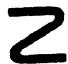
\includegraphics[keepaspectratio]{images/part001_7b053cb2.jpg}}

If R is not open, there are examples where C is closed but R is not Hausdorff (Exercises 10 and 28).

To show that X/R is Hausdorff we can also apply Proposition 5 of no. 1: M and N being two distinct equivalence classes of R it is sufficient that there should be a continuous mapping f of an open subset A of X, saturated with respect to R and containing M and N, into a Hausdorff space \(X'\) , such that 1) f is constant on each equivalence class mod R contained in A, 2) f takes distinct values on M and N. For since \(A/R_{A}\) can be identified with an open subset of X/R (§ 3, no. 6, Proposition 10, Corollary 1), we can apply Proposition 5 of no. 1 to the mapping g: \(A/R_{A} \to X'\) induced by f, since g is continuous (§ 3, no. 4, Proposition 6).

In particular:

PROPOSITION 9. If \(f\) is a continuous mapping of a topological space \(\mathbf{X}\) into a Hausdorff space \(\mathbf{X}'\) , and \(\mathbf{R}\) is the equivalence relation \(f(x) = f(y)\) , then the quotient space \(\mathbf{X} / \mathbf{R}\) is Hausdorff.

PROPOSITION 10. If X is a Hausdorff space, and if X has a continuous section s with respect to the equivalence relation R, then X/R is Hausdorff and s (X/R) is closed in X.

For (§ 3, no. 5) X/R is homeomorphic to the subspace \(s(\mathrm{X}/\mathrm{R})\) of X, which is Hausdorff. Furthermore \(s(\mathrm{X}/\mathrm{R})\) is the set of all \(x \in \mathbf{X}\) such that \(s(\varphi(x)) = x\) , where \(\varphi: \mathbf{X} \to \mathbf{X}/\mathbf{R}\) is the canonical mapping; hence the second assertion follows from no. 1, Proposition 2.

\subsection{REGULAR SPACES}

PROPOSITION 11. The following properties of a topological space X are equivalent:

(O \(_{III}\) ) The set of closed neighbourhoods of any point of X is a fundamental system of neighbourhoods of the point.

\((O_{\mathrm{III}}^{\prime})\) Given any closed subset \(\mathbf{F}\) of \(\mathbf{X}\) and any point \(x \notin \mathbf{F}\) there is a neighbourhood of \(x\) and a neighbourhood of \(\mathbf{F}\) which do not intersect.

\((\mathrm{O}_{\mathrm{III}}) \Longrightarrow (\mathrm{O}_{\mathrm{III}}^{\prime})\) : If \(\mathbf{F}\) is closed and \(x \notin \mathbf{F}\) , then there is a closed neighbourhood \(\mathbf{V}\) of \(x\) contained in the neighbourhood \(\complement \mathbf{F}\) of \(x\) ; \(\mathbf{V}\) and \(\complement \mathbf{V}\) are neighbourhoods of \(x\) and \(\mathbf{F}\) respectively, and have no point in common.

\((\mathrm{O}_{\mathrm{III}}^{\prime}) \Longrightarrow (\mathrm{O}_{\mathrm{III}})\) : If \(W\) is an open neighbourhood of \(x \in X\) , then there is a neighbourhood \(U\) of \(x\) and a neighbourhood \(V\) of \(\complement W\) which are disjoint, and therefore \(\overline{U} \subset W\) .

DEFINITION 2. A topological space is said to be regular if it is Hausdorff and satisfies axiom (O \(_{III}\) ); its topology is then said to be regular.

A discrete space is regular. * We shall see in § 9 that every locally compact space (in particular the real line R) is regular. *

PROPOSITION 12. Every subspace of a regular space is regular.

Let A be a subspace of a regular space X. Since X is Hausdorff, so is A (no. 2); on the other hand, every neighbourhood of a point \(x \in A\) with respect to A is of the form \(V \cap A\) , where V is a neighbourhood of x in X. Since X is regular there is a neighbourhood W of x in X which is closed in X and contained in V; \(W \cap A\) is then a neighbourhood of x in A, closed in A and contained in \(V \cap A\) . Hence the result. Conversely:

PROPOSITION 13. If every point x of a topological space X has a closed neighbourhood which is a regular subspace of X, then X is regular.

X is Hausdorff by Proposition 6 of no. 2. Let x be any point of X and let V be a closed regular neighbourhood of x. If U is any neighbourhood of x contained in V, then U is a neighbourhood of x relative to V; hence by hypothesis there is a neighbourhood W of x in V which is closed in V and contained in U. But W is a neighbourhood of x in X since V is a neighbourhood of x in X, and W is closed in X since V is closed in X.

Remarks. 1) There are examples of non-Hausdorff spaces in which every point has a regular neighbourhood (Exercise 7).

\begin{enumerate}
\def\labelenumi{\arabic{enumi})}
\setcounter{enumi}{1}
\item
  There are spaces which are Hausdorff but not regular (Exercise 20).
\item
  A topology which is finer than a regular topology need not be regular (Exercise 20).
\end{enumerate}

\subsection{EXTENSION BY CONTINUITY; DOUBLE LIMIT}

THEOREM 1. Let X be a topological space, A a dense subset of X, \(f: \mathbf{A} \to \mathbf{Y}\) a mapping of A into a regular space Y. A necessary and sufficient condition for \(f\) to extend to a continuous mapping \(\overline{f}: \mathbf{X} \to \mathbf{Y}\) is that, for each \(x \in \mathbf{X}\) , \(f(y)\) tends to a limit in Y when \(y\) tends to \(x\) while remaining in A. The continuous extension \(\overline{f}\) of \(f\) to X is then unique.

The uniqueness of \(\vec{f}\) follows from the principle of extension of identities (no. 1, Proposition 2, Corollary 1). It is clear that the condition is necessary, for if \(\vec{f}\) is continuous on X, then for each \(x \in X\) we have

\[
\overline {{f}} (x) = \lim _ {y > x, y \in \mathbf {A}} \overline {{f}} (y) = \lim _ {y > x, y \in \mathbf {A}} f (y)
\]

(§ 7, no. 5). Conversely, suppose that the condition is satisfied and define

\[
\overline {{f}} (x) = \lim _ {y \rightarrow x, y \in \mathbf {A}} f (y)
\]

for each \(x \in X\) ; \(\overline{f}(x)\) is a well-defined element of Y, since Y is Hausdorff. We have to show that \(\overline{f}\) is continuous at each point \(x \in X\) . Let then \(V'\) be a closed neighbourhood of \(\overline{f}(x)\) in Y; then by hypothesis there is an open neighbourhood V of x in X such that \(f(V \cap A) \subset V'\) . Since V is a neighbourhood of each of its points, we have

\[
\overline {{f}} (z) = \lim _ {y > z, y \in \mathrm{V} \cap \mathrm{A}} f (y)
\]

for each \(z \in \mathbf{V}\) , and from this it follows that \(\overline{f}(z) \in f(\mathbf{V} \cap \mathbf{A}) \subset \mathbf{V}'\) , since \(\mathbf{V}'\) is closed. The result now follows from the fact that the closed neighbourhoods of \(f(x)\) form a fundamental system of neighbourhoods of \(f(x)\) in \(\mathbf{Y}\) .

The mapping \(\bar{f}\) is said to be obtained by extending f by continuity to X.

In the statement of Theorem 1 the hypothesis that Y is regular cannot be weakened without imposing additional restrictions on X, A or f (Exercise 19).

COROLLARY. Let \(\mathfrak{F}_1\) be a filter on a set \(X_1\) , and \(\mathfrak{F}_2\) a filter on a set \(X_2\) ; let \(\mathfrak{F}_1 \times \mathfrak{F}_2\) be the product filter (§ 6, no. 7) on \(X = X_1 \times X_2\) , and let \(f\) be a mapping of \(X\) into a regular space \(Y\) . Suppose that

\begin{enumerate}
\def\labelenumi{\alph{enumi})}
\item
  \(\lim_{\mathfrak{F}_1\times \mathfrak{F}_2}f\) exists.
\item
  \(\lim_{x_2, \mathfrak{F}_2} f(x_1, x_2) = g(x_1)\) exists for all \(x_1 \in \mathbf{X}_1\) .
\end{enumerate}

Then \(\lim_{x_1, \mathfrak{F}_1} g(x_1)\) exists and is equal to \(\lim_{\mathfrak{F}_1 \times \mathfrak{F}_2} f\) .

Let \(X_1' = X_1 \cup \{ \omega_1 \}\) (resp. \(X_2' = X_2 \cup \{ \omega_2 \}\) ) be the topological space associated with the filter \(\mathfrak{F}_1\) (resp. \(\mathfrak{F}_2\) ) (§ 6, no. 5, Example). In the product space \(X' = X_1' \times X_2'\) let \(X''\) be the union of the subspaces \(X_1 \times X_2'\) and \(\{ (\omega_1, \omega_2) \}\) . \(X\) is clearly a dense subspace of \(X''\) , and the hypotheses imply that \(f(y_1, y_2)\) tends to a limit when \((y_1, y_2)\) tend to any point \((x_1, x_2)\) of \(X''\) whilst remaining in \(X\) . The existence of the extension of \(f\) by continuity to \(X''\) then follows from Theorem 1. Since also \((\omega_1, \omega_2)\) lies in the closure of \(X_1 \times \{ \omega_2 \}\) relative to \(X''\) , the result follows immediately (§ 7, no. 5).

\subsection{EQUIVALENCE RELATIONS ON A REGULAR SPACE}

PROPOSITION 14. Let X be a regular space, R a closed equivalence relation on X. Then the graph C of R in X × X is closed.

Let \((a, b)\) be a point of \(X \times X\) in the closure of C, and let V (resp. W) be a closed neighbourhood of \(a\) (resp. a neighbourhood of \(b\) ) in X; then there is a point \((x, y) \in C \cap (V \times W)\) . Since \(x \in V\) , \(y\) belongs to the saturation S of V with respect to R; hence each neighbourhood W of \(b\) meets S. By hypothesis S is closed, and therefore \(b \in S\) . Now let B be the saturation of \(\{b\}\) with respect to R, then each closed neighbourhood V of \(a\) meets B; since by hypothesis B is closed and X is regular, it follows that \(a \in B\) and therefore that \((a, b) \in C\) . This completes the proof.

COROLLARY. On a regular space, every equivalence relation which is both open and closed is Hausdorff.

This follows from Proposition 14 and Proposition 8 of no. 3.

PROPOSITION 15. Let X be a regular space, F a closed subset of X, R the equivalence relation on X obtained by identifying all the points of F {[}in other words, the equivalence relation whose equivalence classes are F (if \(\mathbf{F} \neq \emptyset\) ) and the sets \(\{x\}\) where \(x \in [\mathbb{C}F]\) . Then the quotient space X/R is Hausdorff.

Let M and N be two distinct equivalence classes in X. If each of them consists of a single point in the complement of F, then there exist two disjoint open neighbourhoods of M and N in the Hausdorff subspace \(\complement F\); these are neighbourhoods of M and N in X and are saturated with respect to R. If M = F (so that \(F \neq \varnothing\) ) and \(N = \{b\}\) where \(b \notin F\) , then since X is regular there is an open neighbourhood of b and an open neighbourhood of F which do not intersect; these neighbourhoods are saturated with respect to R, and the proposition is proved.

Note that the quotient space X/R is not necessarily regular (Chapter IX, § 4, Exercise 14).

\section{COMPACT SPACES AND LOCALLY COMPACT SPACES}

\subsection{QUASI-COMPACT SPACES AND COMPACT SPACES}

DEFINITION 1. A topological space X is said to be quasi-compact if it satisfies the following axiom:

\begin{enumerate}
\def\labelenumi{(\Alph{enumi})}
\setcounter{enumi}{2}
\tightlist
\item
  Every filter on X has at least one cluster point.
\end{enumerate}

A topological space is said to be compact if it is quasi-compact and Hausdorff.

It follows immediately from this axiom that if \(f\) is a mapping of a set \(Z\) into a quasi-compact space \(X\) , and \(\mathfrak{F}\) is any filter on \(Z\) , then \(f\) has at least one cluster point with respect to \(\mathfrak{F}\) . In particular, every sequence of points of a quasi-compact space has at least one cluster point; but this condition is not equivalent to (C) (Exercise 11).

We give three axioms each of which is equivalent to axiom (C):

(C') Every ultrafilter on \(X\) is convergent.

\((\mathrm{C}^{\prime}) \Longrightarrow (\mathrm{C})\) : If \(\mathfrak{F}\) is a filter on \(\mathbf{X}\) then there is an ultrafilter finer than \(\mathfrak{F}\) (§ 6, no. 4, Theorem 1). Since this ultrafilter converges to a point \(x\) , \(x\) is a cluster point of \(\mathfrak{F}\) .

\begin{enumerate}
\def\labelenumi{(\Alph{enumi})}
\setcounter{enumi}{2}
\tightlist
\item
  \(\Longrightarrow\) (C'): For if an ultrafilter has a cluster point then it converges to this point (§ 7, no. 2, Corollary to Proposition 4).
\end{enumerate}

If \(f\) is a mapping of a set \(Z\) into a quasi-compact space \(X\) , and \(\mathfrak{U}\) is an ultrafilter on \(Z\) , \(f\) has at least one limit point with respect to \(\mathfrak{U}\) (§ 6, no. 6, Proposition 10).

(C'') Every family of closed subsets of X whose intersection is empty contains a finite subfamily whose intersection is empty.

\begin{enumerate}
\def\labelenumi{(\Alph{enumi})}
\setcounter{enumi}{2}
\tightlist
\item
  \(\Longrightarrow\) (C'\,'): Let \(\mathfrak{G}\) be a family of closed subsets of X with empty intersection. If every finite subfamily of \(\mathfrak{G}\) has a non-empty intersection, then \(\mathfrak{G}\) generates a filter (§ 6, no. 2, Proposition 1) which has a cluster point by hypothesis. This point belongs to all the sets of \(\mathfrak{G}\) (since they are closed); so we have a contradiction.
\end{enumerate}

\((\mathbf{C}^{\prime\prime}) \Longrightarrow (\mathbf{C}) : \text{For if } (\mathbf{C}) \text{ is false then there is a filter } \mathfrak{F} \text{ on } \mathbf{X} \text{ which has no cluster point; hence the closures of the sets of } \mathfrak{F} \text{ form a family of closed subsets of } \mathbf{X} \text{ contradicting axiom } (\mathbf{C}^{\prime\prime}).\)

(C \(^{iii}\) ) (Axiom of Borel-Lebesgue) Every open covering of X contains a finite open covering of X.

\((\mathbf{C}^{\prime\prime\prime}) \iff (\mathbf{C}^{\prime\prime})\) by taking complements.

If X is quasi-compact, then every locally finite covering R of X is finite. For each point of X has an open neighbourhood which meets only a finite number of sets of R, and by \((\mathbf{C}^{\prime\prime})\) a finite number of these neighbourhoods covers X.

Examples. 1) Every finite space is quasi-compact, and more generally every space in which there is only a finite number of open sets is quasi-compact. A finite space is compact if and only if it is discrete, for a finite Hausdorff space is discrete (§ 8, no.1, Corollary to Proposition 3). Conversely, every compact discrete space is finite, for in such a space the sets consisting of a single point are open; hence the space is finite by (C'\,').

\begin{enumerate}
\def\labelenumi{\arabic{enumi})}
\setcounter{enumi}{1}
\tightlist
\item
  Let X be a set, and give X the topology in which the closed sets are X and all finite subsets of X {[}this set of subsets clearly satisfies axioms \((\mathrm{O}_{\mathrm{I}}^{\prime})\) and \((\mathrm{O}_{\mathrm{II}}^{\prime})\) of §1, no. 4{]}. The topological space so defined is quasi-compact. For if \((\mathbf{F}_{i})_{i\in I}\) is a family of closed subsets of X with empty intersection, then \(F_{\alpha}\) is finite for some \(\alpha\in I\) . Let \(a_{k}\) ( \(1\leqslant k\leqslant n\) ) be the elements of \(F_{\alpha}\) ; then by hypothesis for each index k there is an index \(i_{k}\in I\) such that \(a_{k}\notin F_{i_{k}}\) ; the intersection of the \(F_{i_{k}}\) ( \(1\leqslant k\leqslant n\) ) and \(F_{\alpha}\) is therefore empty, whence axiom \((\mathrm{C}^{\prime\prime})\) is satisfied. If X is infinite it is not Hausdorff.
\end{enumerate}

Remark. Quasi-compact (non-Hausdorff) spaces are of use mainly in applications of topology to algebraic geometry and are seldom featured in other mathematical theories, where on the contrary compact spaces play an important role.

THEOREM 1. Let \(\mathfrak{F}\) be a filter on a quasi-compact space \(\mathbf{X}\) and let \(\mathbf{A}\) be the set of cluster points of \(\mathfrak{F}\) . Then every neighbourhood of \(\mathbf{A}\) belongs to \(\mathfrak{F}\) .

Let V be a neighbourhood of A and suppose it possible that every set of F meets CV. The intersections of the sets of F with CV then form a base of a filter G on X; X is quasi-compact, so that G has at least one cluster point y, which does not belong to A, because the neighbourhood V of A does not meet some of the sets of G. But since G is finer than F, y is also a cluster point of F, which is contrary to hypothesis.

COROLLARY. For a filter on a compact space to converge it is necessary and sufficient that it has a single cluster point.

Necessity by § 8, no. 1, Proposition 1; sufficiency by Theorem 1 above.

\subsection{REGULARITY OF A COMPACT SPACE}

PROPOSITION I. Let X be a compact space, x a point of X. In order that a filter base B formed of closed neighbourhoods of x should be a fundamental system of neighbourhoods of x it is necessary and sufficient that the intersection of the sets of B consists of x alone.

The condition is necessary since X is Hausdorff (§ 8, no. 1, Proposition 1). It is sufficient, for it signifies that x is the only cluster point of B; hence B converges to x by the Corollary to Theorem 1 of no. 1.

COROLLARY. Every compact space is regular.

For it follows from axiom (Hi) (§ 8, no. 1, Proposition 1) that the filter base formed by all the closed neighbourhoods of an arbitrary point of the space satisfies the condition of Proposition 1.

The following proposition amplifies the Corollary to Proposition 1:

PROPOSITION 2. Let X be a compact space and let A, B be two disjoint closed subsets of X. Then there exist two open sets U, V, such that \(U \cap V = \varnothing\) and \(A \subset U\) and \(B \subset V\) .

Suppose the conclusion is false. If every neighbourhood U of A meets every neighbourhood V of B, then the sets \(U \cap V\) form a filter base B on X, which therefore has a cluster point \(x \in X\) . Now x must lie in A, since if y is any point of X not in A there is a neighbourhood of y and a neighbourhood of A which do not intersect, since X is regular, and thus y cannot be a cluster point of B. Similarly x must lie in B and we have a contradiction.

\pandocbounded{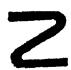
\includegraphics[keepaspectratio]{images/part001_de955d1b.jpg}}

This proposition has important consequences which will be examined in Chapter IX, § 4.

The non-Hausdorff quasi-compact space X of Example 2 of no. 1 does not satisfy axiom (O \(_{III}\) ), nor a fortiori the property stated in Proposition 2, since any two non-empty open sets of this space always intersect.

\subsection{QUASI-COMPACTS SETS; COMPACT SETS; RELATIVELY COMPACT SETS}

DEFINITION 2. A subset A of a topological space X is said to be a quasi-compact (resp. compact) set if the subspace A is quasi-compact (resp. compact).

A subset A of a topological space X is a quasi-compact set if and only if every covering of A by open sets of X contains a finite covering of A; this follows from axiom (C'\,'). In a Hausdorff space, the notions of quasi-compact and compact sets are the same, since every subspace is Hausdorff.

Examples. 1) In a topological space X, every finite subset is quasi-compact; the empty set and every set consisting of one point are compact. 2) In a topological space X, let \((x_{n})_{n\in \mathbb{N}}\) be an infinite sequence of points which converges to a point \(a\) ; then the set A consisting of the points \(x_{n}\) ( \(n\in \mathbb{N}\) ) and \(a\) is quasi-compact. For if \((\mathrm{U}_{\iota})\) is a covering of A by open sets of X, then \(a\in \mathrm{U}_{\iota}\) for some index \(\iota\) . \(\mathrm{U}_{\iota}\) is a neighbourhood of \(a\) and therefore there is only a finite number of indices \(n_k\) such that \(x_{nk}\notin \mathrm{U}_{\iota}\) . For each index \(k\) let \(\iota_{k}\) be an index such that \(x_{nk}\in \mathrm{U}_{\iota_{k}}\) ; then \(\mathrm{U}_{\iota}\) and the \(\mathrm{U}_{\iota_{k}}\) form a finite open covering of A.

PROPOSITION 3. Every closed subset of a quasi-compact (resp. compact) space is quasi-compact (resp. compact).

This is an immediate consequence of axiom (C'') if we remark that if A is closed in X then every set which is closed in A is closed in X.

PROPOSITION 4. Every compact subset of a Hausdorff space is closed.

Let A be a compact subset of a Hausdorff space X, and let x be any point of \(\overline{A}\) ; we have to show that \(x \in A\) . By hypothesis, every neighbourhood of x meets A, and therefore the neighbourhood filter B of x in X induces a filter \(B_{A}\) on A; A is compact whence \(B_{A}\) has a cluster point \(y \in A\) . Since the filter B is coarser than the filter on X generated by \(B_{A}\) (considered as a filter base on X), y is also a cluster point of B; hence y = x, because B converges to x in X and X is Hausdorff (§ 8, no. 1, Proposition 1).

COROLLARY. In a compact space X a subset A is compact if and only if it is closed in X.

PROPOSITION 5. The union of a finite family of quasi-compact subsets of a topological space is quasi-compact.

It is sufficient to show that if A and B are two quasi-compact subsets of a topological space X, then \(A \cup B\) is quasi-compact. Let R be covering of \(A \cup B\) ; then R is a covering of A and a covering of B; hence R contains a finite covering \(R_{1}\) of A and a finite covering \(R_{2}\) of B; \(R_{1} \cup R_{2}\) is thus a finite covering of \(A \cup B\) contained in R.

DEFINITION 3. A subset A of a topological space X is said to be relatively quasi-compact (resp. relatively compact) in X if A is contained in a quasi-compact (resp. compact) subset of X.

To abbreviate, we say also that A is a ``relatively quasi-compact set'' (resp. ``relatively compact set'') when there is no ambiguity about X. In a Hausdorff space the notions of relatively quasi-compact set and relatively compact set are the same.

PROPOSITION 6. If X is a Hausdorff space, a subset A of X is relatively compact if and only if \(\overline{A}\) is compact.

If A is relatively compact, then \(\overline{A}\) is compact by Proposition 4 and its corollary; the reverse implication is self-evident.

PROPOSITION 7. If A is a relatively quasi-compact subset of a topological space X, then every filter base on A has a cluster point in X.

For if \(\mathbf{A} \subset \mathbf{K}\) , where \(\mathbf{K}\) is a quasi-compact subset of \(\mathbf{X}\) , then every filter base on \(\mathbf{A}\) has a cluster point in \(\mathbf{K}\) .

The converse of this proposition is not valid without restriction on X (Exercise 22).

\pandocbounded{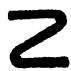
\includegraphics[keepaspectratio]{images/part001_f875b0ae.jpg}}

Remark. In a non-Hausdorff space, a compact set need not be closed, and its closure need not be quasi-compact (Exercise 5); the intersection of two compact sets need not be quasi-compact (Exercise 5); the union of two compact sets need not be compact (Exercise 5).

\subsection{IMAGE OF A COMPACT SPACE UNDER A CONTINUOUS MAPPING}

THEOREM 2. If \(f\) is a continuous mapping of a quasi-compact space \(\mathbf{X}\) into a topological space \(\mathbf{X}'\) , then the set \(f(\mathbf{X})\) is quasi-compact.

Let \(\Re\) be a covering of \(f(\mathbf{X})\) by open sets in \(\mathbf{X}'\) ; then \(\overline{f}^{1}(\Re)\) is an open covering of \(\mathbf{X}\) ( \(\S 2\) , no. 1, Theorem 1); hence there is a finite subset \(\mathfrak{S}\) of \(\Re\) such that \((\mathfrak{S}\overline{f}^{1})\) is a covering of \(\mathbf{X}\) ; but then \(\mathfrak{S}\) is a covering of \(f(\mathbf{X})\) and the theorem is proved.

COROLLARY I. Let \(f\) be a continuous mapping of a topological space \(\mathbf{X}\) into a Hausdorff space \(\mathbf{X}'\) . Then the image under \(f\) of any quasi-compact (resp. relatively quasi-compact) set in \(\mathbf{X}\) is a compact (resp. relatively compact) set in \(\mathbf{X}'\) .

COROLLARY 2. Every continuous mapping \(f\) of a quasi-compact space \(X\) into a Hausdorff space \(X'\) is closed. If also \(f\) is bijective, then \(f\) is a homeomorphism.

This follows immediately from Corollary 1 and Proposition 4 of no. 3.

In particular :

COROLLARY 3. A Hausdorff topology which is coarser than the topology of a quasi-compact space must coincide with the latter.

COROLLARY 4. Let X be a topological space and R a Hausdorff equivalence relation on X.

\begin{enumerate}
\def\labelenumi{\alph{enumi})}
\item
  If there is a quasi-compact set K in X which meets every equivalence class mod R, then X/R is compact and the canonical mapping of \(K/R_{K}\) onto X/R is a homeomorphism.
\item
  If K also meets each equivalence class in only one point, then K is a continuous section of X with respect to the relation R (§ 3, no. 5).
\end{enumerate}

Let \(f\) be the restriction to \(K\) of the canonical mapping \(X \to X / R\) . Since \(X / R\) is Hausdorff it follows from Corollary 1 that \(X / R\) is compact and from Corollary 2 that \(f\) is closed; hence the bijection \(K / R_K \to X / R\) associated with \(f\) is a homeomorphism (§ 5, no. 2, Proposition 3). This deals with a); b) follows immediately, since we now have \(K / R_K = K\) .

\subsection{PRODUCT OF COMPACT SPACES}

THEOREM 3 (Tychonoff). Every product of quasi-compact (resp. compact) spaces is quasi-compact (resp. compact). Conversely, if a product of non-empty spaces is quasi-compact (resp. compact) then each of the factors is quasi-compact (resp. compact).

In view of the characterization of Hausdorff product spaces given in § 8, no. 2, Proposition 7 it is enough to prove the assertions for quasi-compact spaces. If \(\mathbf{X} = \prod_{\iota \in I} \mathbf{X}_{\iota}\) is quasi-compact and non-empty, then \(\mathbf{X}_{\iota}=\mathrm{pr}_{\iota}(\mathbf{X})\) is quasi-compact by reason of Theorem 2 of no. 4. Conversely, suppose the \(X_{\iota}\) are quasi-compact and let U be an ultrafilter on X; then for each \(\iota\in I\) , \(\mathrm{pr}_{\iota}(\mathfrak{U})\) is an ultrafilter base on \(X_{\iota}\) (§ 6, no. 6, Proposition 10) which therefore converges by reason of axiom (C'); hence U is convergent (§ 7, no. 6, Corollary I of Proposition 10) and therefore X is quasi-compact.

COROLLARY. For a subset of a product of topological spaces to be relatively quasi-compact it is necessary and sufficient that each of its projections should be relatively quasi-compact in the corresponding factor.

Necessity follows from Theorem 2 of § 4. To prove sufficiency, let A be a subset of \(\prod_{i} X_{i}\) such that, for each index \(i\) , \(\operatorname{pr}_{i}(A)\) is contained in a quasi-compact subset \(K_{i}\) of \(X_{i}\) ; then A is contained in the quasi-compact subset \(\prod_{i} K_{i}\) of \(\prod_{i} X_{i}\) .

\subsection{INVERSE LIMITS OF COMPACT SPACES}

PROPOSITION 8. Let \((\mathbf{X}_{\alpha}, f_{\alpha \beta})\) be an inverse system of compact spaces indexed by a directed set I such that \(f_{\alpha \alpha}\) is the identity mapping for each \(\alpha \in \mathbf{I}\) . Let \(\mathbf{X} = \varprojlim \mathbf{X}_{\alpha}\) be the inverse limit and \(f_{\alpha}: \mathbf{X} \to \mathbf{X}_{\alpha}\) the canonical mapping (§ 4, no. 4). Then

\begin{enumerate}
\def\labelenumi{\alph{enumi})}
\tightlist
\item
  X is compact and for each \(\alpha \in I\) we have
\end{enumerate}

\[
f _ {\alpha} (\mathbf {X}) = \bigcap_ {\beta \geqslant \alpha} f _ {\alpha \beta} (\mathbf {X} _ {\beta}).\tag{I}
\]

\begin{enumerate}
\def\labelenumi{\alph{enumi})}
\setcounter{enumi}{1}
\tightlist
\item
  If the \(\mathbf{X}_{\alpha}\) are all non-empty then \(\mathbf{X}\) is non-empty.
\end{enumerate}

X is a closed subspace of \(\prod_{\alpha} X_{\alpha}\) (§ 8, no. 2, Proposition 7, Corollary 2)

which is compact by Theorem 3 of no. 5 and Proposition 3 of no. 3. The other assertions are consequences of Set Theory, chap.~III, § 7, no. 4, th. 1. We apply this theorem by taking \(\mathfrak{S}_{\alpha}\) to be the set of closed subsets of \(\mathbf{X}_{\alpha}\) . The conditions (i) and (ii) are just axioms \((\mathrm{O}_{\mathbf{i}}^{\prime})\) and \((\mathbf{C}^{\prime \prime})\) respectively; condition (iii) is satisfied since \(\{x_{\alpha}\}\) is closed and \(f_{\alpha \beta}\) continuous ( \(\S 2\) , no. 1, Theorem 1), and lastly condition (iv) is satisfied by reason of Corollary 2 of Theorem 2 of no. 4.

COROLLARY I. Let \((\mathbf{X}_{\alpha}, f_{\alpha\beta})\) be an inverse system of topological spaces indexed by a directed set, such that for each pair of indices \(\alpha\) , \(\beta\) for which \(\alpha \leqslant \beta\) and for each \(x_{\alpha} \in X_{\alpha}\) , \(\overline{f}_{\alpha\beta}(x_{\alpha})\) is compact. Then equation (1) is valid and \(\overline{f}_{\alpha}(x_{\alpha})\) is compact for each index \(\alpha\) and each \(x_{\alpha} \in X_{\alpha}\) .

For each \(x_{\alpha} \in \bigcap_{\beta \geqslant \alpha} f_{\alpha \beta}(X_{\beta})\) and each \(\beta \geqslant \alpha\) , let \(L_{\beta}\) denote \(\overline{f}_{\alpha \beta}^{1}(x_{\alpha})\) . If \(\alpha \leqslant \beta \leqslant \gamma\) , then we have \(f_{\beta \gamma}(L_{\gamma}) \subset L_{\beta}\) and the set of all indices \(\beta \geqslant \alpha\) is cofinal in the index set. It follows immediately that the \(L_{\beta} (\beta \geqslant \alpha)\) form an inverse system of topological spaces (with the restrictions of the \(f_{\beta \gamma}\) as mappings), whose inverse limit \(L\) is homeomorphic to \(\overline{f}_{\alpha}^{1}(x_{\alpha})\) . Since by hypothesis the \(L_{\beta}\) are compact and not empty, the corollary follows from Proposition 8.

COROLLARY 2. Let \((\mathbf{X}_{\alpha}, f_{\alpha \beta})\) and \((\mathbf{X}_{\alpha}^{\prime}, f_{\alpha \beta}^{\prime})\) be two inverse systems of topological spaces indexed by the same directed set I, and let \((u_{\alpha})\) be an inverse system of mappings \(u_{\alpha}: \mathbf{X}_{\alpha} \to \mathbf{X}_{\alpha}^{\prime}\) . Let \(\mathbf{X} = \varprojlim \mathbf{X}_{\alpha}\) , \(\mathbf{X}^{\prime} = \varprojlim \mathbf{X}_{\alpha}^{\prime}\) , \(u = \varprojlim u_{\alpha}\) . Then:

\begin{enumerate}
\def\labelenumi{\alph{enumi})}
\item
  If \(x' = (x_{\alpha}') \in \mathbf{X}'\) is such that \(\overline{u}_{\alpha}(x_{\alpha}')\) is compact and non-empty for each \(\alpha \in I\) , then \(\overline{u}^1(x')\) is compact and non-empty.
\item
  If the \(X_{\alpha}\) are compact, the \(X_{\alpha}^{\prime}\) Hausdorff and the \(u_{\alpha}\) surjective and continuous, then u is surjective.
\end{enumerate}

Let \(\mathbf{L}_{\alpha}\) denote \(\overline{\boldsymbol{u}}_{\alpha}^{1}(x_{\alpha}^{\prime})\) ; then clearly the \(\mathbf{L}_{\alpha}\) form an inverse system of topological spaces (with the restrictions of the \(f_{\alpha \beta}\) as maps) and \(\overline{\boldsymbol{u}}^{1}(x^{\prime} = \mathbf{L})\) is the inverse limit of the \(\mathbf{L}_{\alpha}\) ; assertion a) therefore follows from Proposition 8. Assertion b) is an immediate consequence, in view of Proposition 3 of no. 3.

\subsection{LOCALLY COMPACT SPACES}

DEFINITION 4. A topological space X is said to be locally compact if it is Hausdorff and if every point of X has a compact neighbourhood.

Clearly a compact space is locally compact, but the converse is false; for example, every discrete space is locally compact, but not compact if infinite.

* As we shall see in Chapter IV, § 2, the real line R is locally compact, but not compact. *

PROPOSITION 9. Every locally compact space is regular.

Let X be a locally compact space, then every point \(x \in X\) has a compact neighbourhood V; since X is Hausdorff, V is closed (no. 3, Proposition 4). On the other hand, V is a regular subspace of X (no. 2, Corollary to Proposition 1) and therefore X is regular (§ 8, no. 4, Proposition 13).

COROLLARY. In a locally compact space every point has a fundamental system of compact neighbourhoods.

For the intersection of a closed neighbourhood of x and a compact neighbourhood of x is a compact neighbourhood of x (no. 3, Proposition 3).

\pandocbounded{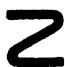
\includegraphics[keepaspectratio]{images/part001_13daf5c9.jpg}}

There exist non-Hausdorff topological spaces in which every point has a fundamental system of compact neighbourhoods (Exercise 5).

The Corollary to Proposition 9 may be generalized as follows:

PROPOSITION 10. In a locally compact space X, every compact set K has a fundamental system of compact neighbourhoods.

Let \(\mathbf{U}\) be any neighbourhood of \(\mathbf{K}\) . For each \(x \in \mathbf{K}\) there is a compact neighbourhood \(\mathbf{W}(x)\) of \(x\) contained in \(\mathbf{U}\) . The interiors of the sets

W (x) form an open covering of K as x runs through K; hence there exist a finite number of points \(x_{i} \in K\) ( \(1 \leqslant i \leqslant n\) ) such that the interiors of the \(W(x_{i})\) cover K. The union V of the \(W(x_{i})\) is therefore a compact neighbourhood of K contained in U (no. 3, Proposition 5).

PROPOSITION 11. Let X be a locally compact space and F a subset of X such that \(F \cap K\) is compact whenever K is a compact subset of X. Then F is closed in X.

In view of Proposition 4 of no. 3, this follows from Proposition 3 a) of § 3, no. 1.

PROPOSITION 12. In a Hausdorff space X, every locally compact subspace A is locally closed.

By hypothesis, for every \(x \in A\) there is a neighbourhood V of x in X such that \(V \cap A\) is compact and therefore closed in V (no. 3, Proposition 4).

PROPOSITION 13. Every locally closed subspace of a locally compact space X is locally compact.

Let A be a locally closed subspace of X; then for each \(x \in A\) there is a neighbourhood U of x in X such that \(U \cap A\) is closed in U. Let \(V \subset U\) be a compact neighbourhood of x in X; \(V \cap A = V \cap (U \cap A)\) is closed in V and therefore compact (no. 3, Proposition 3). Since \(V \cap A\) is a neighbourhood of x in A, the result is proved (it is clear that A is Hausdorff).

\pandocbounded{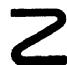
\includegraphics[keepaspectratio]{images/part001_5df2d3a1.jpg}}

Theorem 1 (no. 1) and Corollary 2 of Theorem 2 (no. 4) do not extend to locally compact spaces which are not compact.

For example, in an infinite discrete space X, the filter consisting of those sets which contain a given point \(x \in X\) and have a finite complement has x as its only cluster point but does not converge to x. Since any mapping f of X into a Hausdorff space \(X'\) is continuous, the image under f of an arbitrary subset of X (which is closed in X, since X is discrete) will not in general be a closed subset of \(X'\) .

The proposition corresponding to Theorem 3 of no. 5 is the following:

PROPOSITION 14. a) Let \((\mathbf{X}_{\iota})_{\iota \in I}\) be a family of locally compact spaces such that \(\mathbf{X}_{\iota}\) is compact for all but a finite number of indices. Then the product space \(\mathbf{X} = \prod_{\iota \in I} \mathbf{X}_{\iota}\) is locally compact.

\begin{enumerate}
\def\labelenumi{\alph{enumi})}
\setcounter{enumi}{1}
\item
  Conversely, if the product of a family \((\mathbf{X}_{\iota})_{\iota\in I}\) of non-empty topological spaces is locally compact, then the factors \(\mathbf{X}_{\iota}\) are compact for all but a finite number of indices, and the factors which are not compact are locally compact.
\item
  Let \(x = (x_{\iota})\) be a point of \(X\) . For each index \(\iota \in I\) such that \(X_{\iota}\) is locally compact but not compact, let \(V_{\iota}\) be a compact neighbourhood of \(x_{\iota}\) in \(X_{\iota}\) , and for all other indices \(\iota\) put \(V_{\iota} = X_{\iota}\) . Then \(\prod_{\iota \in I} V_{\iota}\) is a compact neighbourhood of \(x\) in \(X\) (no. 5, Theorem 3). Also \(X\) is Hausdorff by § 8, no. 2, Proposition 7, and is therefore locally compact.
\item
  If \(X = \prod_{\iota \in I} X_{\iota}\) is locally compact and the \(X_{\iota}\) non-empty, then each of the \(X_{\iota}\) is homeomorphic to a closed subspace of \(X\) (§ 4, no. 2, Proposition 4 and § 4, no. 3, Corollary to Proposition 7), hence locally compact by Proposition 13. Let \(a = (a_{\iota})\) be a point of \(X\) and let \(V\) be a compact neighbourhood of \(a\) ; since we have \(pr_{\iota}V = X_{\iota}\) for all but a finite number of indices (§ 4, no. 1), it follows from no. 4, Corollary 1 to Theorem 2, that the \(X_{\iota}\) are compact except for a finite number of indices.
\end{enumerate}

\subsection{EMBEDDING OF A LOCALLY COMPACT SPACE IN A COMPACT SPACE}

THEOREM 4 (Alexandroff). If X is any locally compact space, there exists a compact space \(X'\) and a homeomorphism f of X onto the complement of a point in \(X'\) . Furthermore, if \(X_{1}'\) is another compact space such that there is a homeomorphism \(f_{1}\) of X onto the complement of a point in \(X_{1}'\) , then there is a unique homeomorphism g of \(X'\) onto \(X_{1}'\) such that \(f_{1}=g\circ f\) .

Let us begin by proving the second assertion of the theorem. Let

\[
f (\mathbf {X}) = \mathbf {X} ^ {\prime} - \left\{\omega \right\} \quad \text { and } \quad f _ {1} (\mathbf {X}) = \mathbf {X} _ {1} ^ {\prime} - \left\{\omega_ {1} \right\}.
\]

If the homeomorphism \(g\) exists it must be unique, for by definition we have \(g(x') = f_1(\overline{f}^1 (x'))\) if \(x' \neq \omega\) and therefore \(g(\omega) = \omega_1\) . It remains to show that the bijection \(g: \mathbf{X}' \to \mathbf{X}_1'\) thus defined is bicontinuous; since \(\mathbf{X}'\) and \(\mathbf{X}_1'\) are interchangeable we need only show that the image under \(g\) of a neighbourhood of a point \(x' \in \mathbf{X}'\) is a neighbourhood of \(g(x')\) in \(\mathbf{X}_1'\) . This is obvious from the definition of \(g\) if \(x' \neq \omega\) . If \(x' = \omega\) , let \(V'\) be an open neighbourhood of \(\omega\) in \(X'\) ; then \(X' - V' = K\) is closed in \(X'\) and therefore compact (no. 3, Proposition 3) and is contained in \(f(X)\) ; hence \(g(K) = f_1(\overline{f}^1 (K))\) is compact (no. 4, Theorem 2, Corollary 1). It follows that \(g(V') = X_1' - g(K)\) is an open neighbourhood of \(\omega_1\) (no. 3, Proposition 4). Hence \(g\) is a homeomorphism.

To prove the first part of the theorem, let \(X'\) be a set which is the sum of X and a set consisting of a single point \(\omega\) . We define a topology on \(X'\) by taking the set D of open subsets of \(X'\) to consist of all open subsets of X and all subsets of the form \((\mathbf{X}-\mathbf{K})\cup\{\omega\}\) , where K is a compact subset of X. Since any intersection of compact subsets of X is compact (no. 3, Propositions 3 and 4) and since any closed subset of a compact set is compact (no. 3, Proposition 3), it follows that \(\mathfrak{D}\) satisfies axiom \((\mathrm{O_I})\) ; and since any finite union of compact subsets of X is compact (no. 3, Proposition 5), \(\mathfrak{D}\) also satisfies \((\mathrm{O_{II}})\) . Every compact subset of X is closed in X (no. 3, Proposition 4) and therefore the topology induced on X by that of \(\mathbf{X}'\) is the original topology on X. Thus it remains to show that \(\mathbf{X}'\) is compact. In the first place, \(\mathbf{X}'\) is Hausdorff. For if \(x, y\) are any two distinct points of X, they have disjoint open neighbourhoods V, W respectively in X, and V, W are open in \(\mathbf{X}'\) ; on the other hand each \(x \in \mathbf{X}\) has a compact neighbourhood K in X, which is also a neighbourhood of \(x\) in \(\mathbf{X}'\) , while

\[
(\mathbf {X} - \mathbf {K}) \cup \{\omega \}
\]

is a neighbourhood of \(\omega\) in \(\mathbf{X}'\) and manifestly does not meet \(\mathbf{K}\) . Finally, \(\mathbf{X}'\) is quasi-compact. Let \((\mathbf{U}_{\lambda})_{\lambda \in \mathbf{L}}\) be an open covering of \(\mathbf{X}'\) ; then for at least one index \(\mu \in \mathbf{L}\) we have \(\mathbf{U}_{\mu} = (\mathbf{X} - \mathbf{K}_{\mu}) \cup \{\omega\}\) where \(\mathbf{K}_{\mu}\) is a compact subset of \(\mathbf{X}\) . Hence there is a finite subset \(\mathbf{H}\) of \(\mathbf{L}\) such that the sets \(\mathbf{U}_{\lambda}\) (for \(\lambda \in \mathbf{H}\) ) cover \(\mathbf{K}_{\mu}\) ; if \(\mathbf{J} = \mathbf{H} \cup \{\mu\}\) , then \((\mathbf{U}_{\lambda})_{\lambda \in \mathbf{J}}\) is a finite open covering of \(\mathbf{X}'\) , and the proof is complete.

Notice that if X is already compact, then \(\omega\) is an isolated point of the compact space \(X'\) ; hence \(X'\) is the sum ( \(\S\) 2, no. 4, Example 3) of the space X and the space \(\{\omega\}\) .

When a compact space \(X'\) has been constructed as above from a locally compact space X by adjoining an element \(\omega\) , it is often said that \(\omega\) is the ``point at infinity'' of \(X'\) , and that \(X'\) is obtained from X by adjoining a point at infinity. \(X'\) is also called the Alexandroff compactification or the one-point compactification of the locally compact space X.

* Example. If we apply Alexandroff's theorem to the real plane \(\mathbf{R}^2\) , we get a compact space homeomorphic to the sphere \(\mathbf{S}_2\) whose equation is \(x_1^2 + x_2^2 + x_3^2 = 1\) in \(\mathbf{R}^3\) . A homeomorphism of these two spaces may be described as follows: the point \(\omega\) (the point at infinity) adjoined to \(\mathbf{R}^2\) is mapped to \((0, 0, 1) \in \mathbf{S}_2\) , and every point \((x_1, x_2)\) of \(\mathbf{R}^2\) is mapped to the point where the line joining the points \((0, 1, 1)\) and \((x_1, x_2, 0)\) in \(\mathbf{R}^3\) meets \(\mathbf{S}_2\) again. This homeomorphism is known as stereographic projection.

\subsection{LOCALLY COMPACT σ-COMPACT SPACES}

DEFINITION 5. A locally compact space X is said to be σ-compact or countable at infinity if it is a countable union of compact subsets.

Examples. 1) A discrete space is \(\sigma\) -compact if and only if it is countable. *2) The real line \(\mathbf{R}\) is locally compact and \(\sigma\) -compact, since it is the union of the compact intervals \([-n, +n]\) for \(n \in \mathbb{N}\) . *

\pandocbounded{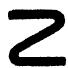
\includegraphics[keepaspectratio]{images/part001_9ca68205.jpg}}

Remark. A Hausdorff space can be a countable union of compact subspaces without being locally compact. * An example is Hilbert space with the weak topology, as we shall show in a later volume.

PROPOSITION 15. If X is a locally compact \(\sigma\) -compact space, there is a sequence \((\mathbf{U}_n)\) of relatively compact open subsets of X which cover X, such that \(\overline{\mathbf{U}}_n \subset \mathbf{U}_{n+1}\) for each \(n\) .

Let X be the union of a sequence \((\mathbf{K}_{n})\) of compact sets. Let \(U_{1}\) be a relatively compact open neighbourhood of \(K_{1}\) (no. 7, Proposition 10) and define \(U_{n}\) inductively for n \textgreater{} 1 to be a relatively compact open neighbourhood of \(\overline{U}_{n-1} \in K_{n}\) (no. 3, Proposition 5; no. 7, Proposition 10). The sequence \((\mathbf{U}_{n})\) clearly has the required properties.

COROLLARY I. With the notation of Proposition 15, every compact subset K of X is contained in some \(U_{n}\) .

For K can be covered by a finite number of the \(U_{k}\) , by axiom (C'\,').

COROLLARY 2. Let X be a locally compact space and let X' be the compact space obtained by adjoining a point at infinity ω to X (no. 8). Then X is σ-compact if and only if the point ω has a countable fundamental system of neighbourhoods in X'.

If X is σ-compact we can construct a sequence of subsets \(U_{n}\) of X as in Proposition 15, and the neighbourhoods \(X^{\prime}-\overline{U}_{n}\) of \(\omega\) in \(X^{\prime}\) form a fundamental system of neighbourhoods of \(\omega\) by reason of Corollary 1. The converse follows from the fact that the complements of open neighbourhoods of \(\omega\) are compact subsets of X.

Clearly every closed subspace of a locally compact \(\sigma\) -compact space is locally compact and \(\sigma\) -compact. Likewise any finite product of locally compact \(\sigma\) -compact spaces is locally compact and \(\sigma\) -compact.

Notice, however, that an open subspace of a compact space need not be \(\sigma\) -compact, as Alexandroff's theorem (no. 8, Theorem 4) shows.

\subsection{PARACOMPACT SPACES}

DEFINITION 6. A topological space is said to be paracompact if it is Hausdorff and satisfies the following axiom:

(PC) Every open covering \(\Re\) of X has a locally finite open refinement \(\Re'\) . (Set Theory, Chapter II, § 4, no. 6, Definition 5).

Every compact space is clearly paracompact. Every discrete space X is paracompact, for the open covering formed by all sets consisting of a single point of X is locally finite and is finer than every open covering of X.

PROPOSITION 16. Every closed subspace F of a paracompact space X is paracompact.

Certainly F is Hausdorff. On the other hand, if \((\mathbf{V}_{\iota})\) is an open covering in the subspace F, then each \(V_{\iota}\) is of the form \(V_{\iota} = U_{\iota} \cap F\) , where \(U_{\iota}\) is open in X. Consider the open covering R of X formed by \(\complement F\) and the \(U_{\iota}\) ; since X is paracompact, R has a locally finite refinement \(R'\) , and the intersections with F of the sets belonging to \(R'\) form a locally finite open covering of F which is finer than the given covering \((\mathbf{V}_{\iota})\) .

On the other hand an open subspace of a compact space need not be paracompact (Exercise 11).

PROPOSITION 17. The product of a paracompact space and a compact space is paracompact.

Let X be a paracompact space, Y a compact space, R an open covering of \(X \times Y\) . For each \((x, y) \in X \times Y\) there is an open neighbourhood \(V(x, y)\) of x in X and an open neighbourhood \(W(x, y)\) of y in Y such that \(V(x, y) \times W(x, y)\) is contained in some set belonging to R. For each \(x \in X\) , the sets \(W(x, y)\) as y runs through Y form an open covering of Y; hence there exist a finite number of points

\[
y _ {i} \in Y \quad (1 \leqslant i \leqslant n (x))
\]

such that the \(\mathbf{W}(x, y_i)\) cover \(\mathbf{Y}\) . Let \(\mathbf{U}(x)\) denote

\[
\bigcap_ {i = 1} ^ {n (x)} \mathrm{V} (x, y _ {i});
\]

then each of the open sets \(\mathbf{U}(x) \times \mathbf{W}(x, y_i)\) is contained in a set of \(\Re\) . Now let \((\mathbf{T}_{\iota})_{\iota \in \mathbf{I}}\) be a locally finite open covering of \(\mathbf{X}\) which refines the covering \((\mathbf{U}(x))_{x \in \mathbf{X}}\) . For each \(\iota \in \mathbf{I}\) , let \(x_{\iota}\) be a point of \(\mathbf{X}\) such that \(\mathbf{T}_{\iota} \subset \mathbf{U}(x_{\iota})\) , and let us denote by \(\mathbf{S}_{\iota,k}\) the sets \(\mathbf{W}(x_{\iota}, y_k)\) corresponding to this point \(x_{\iota}\) ( \(1 \leqslant k \leqslant n(x_{\iota})\) ). Clearly the sets

\[
\mathrm{T} _ {\iota} \times \mathrm{S} _ {\iota, k} \quad (\iota \in \mathrm{I}, 1 \leqslant k \leqslant n (x _ {\iota}) \text {   for   each   } \iota \in \mathrm{I})
\]

form an open covering of \(\mathbf{X} \times \mathbf{Y}\) which refines \(\Re\) , and the proof will be complete if we show that this covering is locally finite. Let \((x, y)\) be any point of \(\mathbf{X} \times \mathbf{Y}\) ; there is a neighbourhood \(\mathbf{Q}\) of \(x\) which meets only a finite number of sets \(\mathbf{T}_{\iota}\) , and therefore the neighbourhood \(\mathbf{Q} \times \mathbf{Y}\) of \((x, y)\) meets only a finite number of sets \(\mathbf{T}_{\iota} \times \mathbf{S}_{\iota,k}\) .

On the other hand the product of two paracompact spaces need not be paracompact (see Chapter IX, § 5, Exercise 16).

PROPOSITION 18. The sum (§ 2, no. 4, Example 3) of a family \((\mathbf{X}_{\iota})_{\iota\in I}\) of paracompact spaces is paracompact.

Let X be the sum of the \(X_{\iota}\) , and let \((\mathrm{V}_{\lambda})_{\lambda\in\mathbf{L}}\) be an open covering of X. The covering formed by the open sets \(X_{\iota}\cap V_{\lambda}\) is finer than \((\mathrm{V}_{\lambda})\) . For each \(\iota\in I\) , let \((\mathrm{U}_{\iota,\mu})_{\mu\in\mathbf{M}_{\iota}}\) be a locally finite open refinement of the covering \((\mathrm{V}_{\lambda}\cap\mathrm{X}_{\iota})_{\lambda\in\mathbf{L}}\) ; then the open covering of X formed by the

\[
\mathbf {U} _ {\iota , \mu} \quad (\iota \in \mathbf {I}, \mu \in \mathbf {M} _ {\iota} \text {   for   each   } \iota \in \mathbf {I})
\]

is locally finite and refines the original covering \((\mathbf{V}_{\lambda})\) .

THEOREM 5. A locally compact space X is paracompact if and only if X is the sum of a family of locally compact σ-compact spaces.

Suppose X is paracompact, and for each \(x \in X\) let \(V_x\) be a relatively compact open neighbourhood of x in X. Then by hypothesis there exists a locally finite open covering \((\mathrm{U}(\alpha))_{\alpha \in \Lambda}\) of X which refines the covering \((\mathrm{V}_x)_{x \in \mathbf{X}}\) . The \(\mathrm{U}(\alpha)\) are therefore relatively compact. Every compact subset K of X meets only a finite number of the sets \(\mathrm{U}(\alpha)\) , for the non-empty sets \(\mathrm{U}(\alpha) \cap \mathrm{K}\) form a locally finite open covering of the compact space X; hence they must be finite in number (no. 1). Now let R be the following relation between two points x, y of X: ``there exists a finite sequence \((\alpha_i)_{1 \leqslant i \leqslant n}\) of indices in A such that \(x \in \mathrm{U}(\alpha_1)\) , \(y \in \mathrm{U}(\alpha_n)\) and \(\mathrm{U}(\alpha_i)\) meets \(\mathrm{U}(\alpha_{i+1})\) for \(1 \leqslant i \leqslant n - 1\)''. It is immediately verified that R is an equivalence relation, and that each equivalence class mod R is an open subset of X {[}since the \(\mathrm{U}(\alpha)\) are open sets{]}. X is therefore the sum of the locally compact subspaces (no. 7, Proposition 13) formed by the equivalence classes mod R, and it remains to show that each of these subspaces is the union of a countable subfamily of the family \((\mathrm{U}(\alpha))\) .

Let \(x\) be any point of \(\mathbf{X}\) , and define a sequence \((\mathbf{C}_n)\) of relatively compact open subsets of \(\mathbf{X}\) by induction on \(n\) as follows; \(\mathbf{C}_1\) is the union of the sets \(\mathbf{U}(\alpha)\) which contain \(x\) , and for each \(n > 1\) , \(\mathbf{C}_n\) is the union of the sets \(\mathbf{U}(\alpha)\) which meet \(\mathbf{C}_{n-1}\) . It is immediately verified by induction on \(n\) that each of the \(\mathbf{C}_n\) is relatively compact and is the union of a finite number of sets \(\mathbf{U}(\alpha)\) . Furthermore, the equivalence class of \(x\) with respect to \(\mathbf{R}\) is the union of the \(\mathbf{C}_n\) : for if \((\alpha_i)_{1 \leqslant i \leqslant n}\) is a sequence of indices such that \(x \in \mathbf{U}(\alpha_1)\) and \(\mathbf{U}(\alpha_i)\) meets \(\mathbf{U}(\alpha_{i+1})\) for \(1 \leqslant i \leqslant n - 1\) , then one sees by induction on \(i\) that \(\mathbf{U}(\alpha_i) \subset \mathbf{C}_i\) for \(1 \leqslant i \leqslant n\) . It follows that the equivalence classes mod \(\mathbf{R}\) are \(\sigma\) -compact, and this completes the proof of the first part of the theorem.

To prove the converse, we may assume (by Proposition 18) that X is σ-compact. Let \(\Re = (G_{\lambda})_{\lambda \in L}\) be any open covering of X, and let \((U_n)\) be a sequence of relatively compact open sets in X which have the properties stated in Proposition 15 of no. 9. Let \(K_n\) denote the compact set \(\overline{U}_n - U_{n-1}(U_n = \emptyset\) if \(n \leqslant 0)\) . The open set \(U_{n+1} - \overline{U}_{n-2}\) is a neighbourhood of \(K_n\) by construction; hence for each \(x \in K_n\) there is a neighbourhood \(W_x\) of \(x\) contained in one of the sets \(G_{\lambda}\) and contained also in \(U_{n+1} - \overline{U}_{n-2}\) . Since \(K_n\) is compact, a finite number of the sets \(W_x\) cover \(K_n\) ; let \(H_{ni}(1 \leqslant i \leqslant p_n)\) be these sets. Then the family \(\Re'\) of sets \(H_{ni}(n \geqslant 1, 1 \leqslant i \leqslant p_n\) for each \(n\) ) is an open covering of X which refines \(\Re\) , and hence to complete the proof we have to show that \(\Re'\) is locally finite. Let \(z\) be any point of X, \(n\) the smallest integer such that \(z \in U_n\) ; then since \(z \notin U_{n-1}\) , there is a neighbourhood T of \(z\) which is contained in \(U_n\) and does not meet \(U_{n-2}\) . It follows that T meets only those sets \(H_{mi}\) for which \(n - 2 \leqslant m \leqslant n + 1\) , i.e.~T meets only a finite number of sets of \(\Re'\) .

In the course of the proof we have also established the following result:

COROLLARY. Let X be a locally compact paracompact space. Then every open covering R of X has a locally finite open refinement R' formed of relatively compact sets. If X is σ-compact then R' can be taken to be countable.

\section{PROPER MAPPINGS}

In this section we denote by \(\iota_{\mathbf{X}}\) the identity mapping of a set \(\mathbf{X}\) onto itself.

\subsection{PROPER MAPPINGS}

If \(f: \mathbf{X} \to \mathbf{Y}\) and \(f': \mathbf{X}' \to \mathbf{Y}'\) are two continuous closed mappings, the product \(f \times f': \mathbf{X} \times \mathbf{X}' \to \mathbf{Y} \times \mathbf{Y}'\) is not necessarily a closed map, even if \(f\) is of the form \(\iota_{\mathbf{X}}\) .

Example. Every constant mapping into a Hausdorff space is closed. But if \(f\) is the constant mapping \(\mathbf{Q} \to 0\) , then \(f \times \iota_{\mathbf{Q}}\) is the mapping \((x, y) \to (0, y)\) of \(\mathbf{Q}^2\) into \(\mathbf{Q}^2\) , so it is the second projection and is not closed (§ 4, no. 2, Remark 1).

DEFINITION 1. Let \(f\) be a mapping of a topological space \(\mathbf{X}\) into a topological space \(\mathbf{Y}\) . \(f\) is said to be proper if \(f\) is continuous and if the mapping \(f \times \iota_{\mathbf{Z}} : \mathbf{X} \times \mathbf{Z} \to \mathbf{Y} \times \mathbf{Z}\) is closed, for every topological space \(\mathbf{Z}\) .

We shall give other characterizations of proper mappings in no. 2 and 3.

If in Definition 1 we take the space Z to consist of a single point, we see that:

PROPOSITION 1. Every proper mapping is closed.

PROPOSITION 2. Let \(f: \mathbf{X} \to \mathbf{Y}\) be a continuous injection. Then the following three statements are equivalent:

\begin{enumerate}
\def\labelenumi{\alph{enumi})}
\item
  \(f\) is proper.
\item
  \(f\) is closed.
\item
  \(f\) is a homeomorphism of \(\mathbf{X}\) onto a closed subset of \(\mathbf{Y}\) .
\end{enumerate}

We have just seen that a) implies b). Since the equivalence relation \(f(x) = f(x')\) is the equality relation, the quotient space of X with respect to this relation can be identified with X; hence b) implies c) by reason of § 5, no. 2, Proposition 3. Finally, if c) is satisfied then \(f \times \iota_{\mathbf{Z}}\) is a homeomorphism of \(\mathbf{X} \times \mathbf{Z}\) onto a closed subspace of \(\mathbf{Y} \times \mathbf{Z}\) and is therefore a closed mapping; hence c) implies a).

PROPOSITION 3. Let \(f: \mathbf{X} \to \mathbf{Y}\) be a continuous mapping. If \(\mathbf{T}\) is any subset of \(\mathbf{Y}\) , let \(f_{\mathbf{T}}\) denote the mapping \(\overline{f}^{1}(\mathbf{T}) \to \mathbf{T}\) which agrees with \(f\) on \(\overline{f}^{1}(\mathbf{T})\) .

\begin{enumerate}
\def\labelenumi{\alph{enumi})}
\item
  If \(f\) is proper, so is \(f_{\mathbf{T}}\) .
\item
  Let \((\mathrm{T}(\iota))_{\iota\in I}\) be a family of subsets of Y whose interiors cover Y, or which is a locally finite closed covering of Y; then if each of the mappings \(f_{\mathbf{T}(\iota)}\) is proper, so is \(f\) .
\end{enumerate}

Let \(\mathbf{Z}\) be a topological space. If \(\mathbf{T}\) is any subset of \(\mathbf{Y}\) , we have

\[
f _ {\mathbf {T}} \times \iota_ {\mathbf {Z}} = (f \times \iota_ {\mathbf {Z}}) _ {\mathbf {T} \times \mathbf {Z}};
\]

if \(f\) is proper, then \(f \times \iota_{\mathbf{Z}}\) is closed, hence so is \((f \times \iota_{\mathbf{Z}})_{\mathbf{T} \times \mathbf{Z}}\) {[}§ 5, no. 1, Proposition 2 a){]}, whence a) is proved. If now \((\mathrm{T}(\iota))_{\iota \in \mathbf{I}}\) satisfies one of the two conditions stated in b), then the covering \((\mathrm{T}(\iota) \times \mathbf{Z})_{\iota \in \mathbf{I}}\) of \(\mathbf{Y} \times \mathbf{Z}\) has the same property; if the \(f_{\mathbf{T}(\iota)}\) are proper then the mappings

\[
(f \times \iota_ {\mathbf {Z}}) _ {\mathbf {T} (\iota) \times \mathbf {Z}}
\]

are closed, whence \(f \times \iota_{\mathbf{Z}}\) is closed {[}§ 5, no. 1, Proposition 2 b){]}. This completes the proof.

PROPOSITION 4. Let I be a finite set and for each \(i \in I\) let \(f_i: X_i \to Y_i\) be a continuous mapping. Let \(X = \prod_{i \in I} X_i\) , \(Y = \prod_{i \in I} Y_i\) , and let \(f: X \to Y\)

be the product mapping \((x_{i})\to (f_{i}(x_{i}))\) . Then:

\begin{enumerate}
\def\labelenumi{\alph{enumi})}
\item
  If each of the \(f_i\) is proper, then \(f\) is proper.
\item
  If \(f\) is proper and if the \(X_i\) are non-empty, then each of the \(f_i\) is proper.
\end{enumerate}

(We shall see in no. 2, Theorem 1, Corollary 3, that this proposition extends to infinite products.)

By induction it is enough to consider the case where \(\mathbf{I} = \{\mathbf{1},\mathbf{2}\}\) . a) Suppose that \(f_{1}, f_{2}\) are proper, and let \(\mathbf{Z}\) be a topological space; \(f_{1} \times f_{2} \times \iota_{\mathbf{Z}}\) is the composition of \(\iota_{\mathbf{Y}_1} \times f_2 \times \iota_{\mathbf{Z}}\) and

\[
f _ {1} \times \iota_ {\mathbf {X} _ {2}} \times \iota_ {\mathbf {Z}};
\]

these two mappings are closed by hypothesis, hence so is \(f_{1} \times f_{2} \times \iota_{\mathbf{Z}}\) {[}§ 5, no. 1, Proposition 1 a){]}, whence \(f_{1} \times f_{2}\) is proper.

\begin{enumerate}
\def\labelenumi{\alph{enumi})}
\setcounter{enumi}{1}
\tightlist
\item
  Now suppose \(f\) is proper. Let \(\mathbf{F}\) be a closed subset of \(\mathbf{X}_2 \times \mathbf{Z}\) and let \(\mathbf{G}\) be the image of \(\mathbf{F}\) in \(\mathbf{Y}_2 \times \mathbf{Z}\) under the mapping \(f_2 \times \iota_{\mathbf{Z}}\) . Then the image of \(\mathbf{X}_1 \times \mathbf{F}\) in \(\mathbf{Y}_1 \times \mathbf{Y}_2 \times \mathbf{Z}\) under \(f_1 \times f_2 \times \iota_{\mathbf{Z}}\) is \(f_1(\mathbf{X}_1) \times \mathbf{G}\) . By hypothesis, this is closed in \(\mathbf{Y}_1 \times \mathbf{Y}_2 \times \mathbf{Z}\) ; if \(\mathbf{X}_1 \neq \emptyset\) , then \(f_1(\mathbf{X}_1)\) is not empty, which implies that \(\mathbf{G}\) is closed in \(\mathbf{Y}_2 \times \mathbf{Z}\) (§ 4, no. 3, Corollary to Proposition 7); hence \(f_2\) is proper. Similarly \(f_1\) is proper if \(\mathbf{X}_2 \neq \emptyset\) .
\end{enumerate}

PROPOSITION 5. Let \(f: \mathbf{X} \to \mathbf{X}'\) and \(g: \mathbf{X}' \to \mathbf{X}''\) be two continuous mappings.

\begin{enumerate}
\def\labelenumi{\alph{enumi})}
\item
  If \(f\) and \(g\) are proper, then \(g \circ f\) is proper.
\item
  If \(g \circ f\) is proper and \(f\) is surjective, then \(g\) is proper.
\item
  If \(g \circ f\) is proper and \(g\) is injective, then \(f\) is proper.
\item
  If \(g \circ f\) is proper and \(X'\) is Hausdorff, then \(f\) is proper.
\end{enumerate}

Let \(\mathbf{Z}\) be a topological space. We have

\[
(g \circ f) \times \iota_ {\mathbf {Z}} = (g \times \iota_ {\mathbf {Z}}) \circ (f \times \iota_ {\mathbf {Z}});
\]

if \(f\) and \(g\) are proper, then \(f \times \iota_{\mathbf{Z}}\) and \(g \times \iota_{\mathbf{Z}}\) are closed; hence {[}§ 5, no. 1, Proposition 1 a){]} ( \(g \circ f\) ) × \(\iota_{\mathbf{Z}}\) is closed; this proves a). The proof of b) {[}resp. c){]} runs along the same lines, using part b) {[}resp. c){]} of Proposition 1 of § 5, no. 1, and remarking that if \(f\) is surjective (resp. if \(g\) is injective) then \(f \times \iota_{\mathbf{Z}}\) is surjective (resp. \(g \times \iota_{\mathbf{Z}}\) is injective). Finally, to prove d), consider the commutative diagram

\[
\mathbf {X} \stackrel {\varphi} {\rightarrow} \mathbf {X} \times \mathbf {X} ^ {\prime}\tag{1}
\]

\[
\begin{array}{c} f \downarrow \\ \mathbf {X} ^ {\prime} \xrightarrow [ \psi ]{} \mathbf {X} ^ {\prime \prime} \end{array} \begin{array}{c} \downarrow (g \circ f) \times \iota_ {\mathbf {x} ^ {\prime}} \\ \times \mathbf {X} ^ {\prime} \end{array}
\]

where \(\varphi(x) = (x, f(x))\) and \(\psi(x') = (g(x'), x')\) . The mapping \(\varphi\) (resp. \(\psi\) ) is a homeomorphism of X (resp. X') onto the graph of \(f\) (resp. the reflection of the graph of \(g\) ) ( \(\S 4\) , no. 1, Proposition 1, Corollary 2). Further, since X' is Hausdorff, the graph \(\varphi(X)\) of \(f\) is closed in X × X' ( \(\S 8\) , no. 1, Proposition 2, Corollary 2). Hence (Proposition 2) \(\varphi\) is proper; on the other hand Proposition 4 shows that ( \(g \circ f\) ) × \(\iota_{X'}\) is proper. By a) above and the commutativity of the diagram (1), \(\psi \circ f\) is proper; but \(\psi\) is injective and therefore \(f\) is proper by c) above.

Remark. If \(\mathbf{X}'\) is not Hausdorff it can happen that \(g \circ f\) is proper and \(f\) not; for example, take \(\mathbf{X}\) and \(\mathbf{X}''\) to consist of one point and \(\mathbf{X}'\) to consist of two points, with the coarsest topology.

COROLLARY I. If \(f: \mathbf{X} \to \mathbf{Y}\) is a proper mapping, then the restriction of \(f\) to a closed subset \(\mathbf{F}\) of \(\mathbf{X}\) is a proper mapping of \(\mathbf{F}\) into \(\mathbf{Y}\) .

For this restriction is the composition \(f \circ j\) , where \(j: \mathbf{F} \to \mathbf{X}\) is the canonical injection, which is proper by Proposition 2.

COROLLARY 2. Let \(f: \mathbf{X} \to \mathbf{Y}\) be a proper mapping, where \(\mathbf{X}\) is Hausdorff. Then the subspace \(f(\mathbf{X})\) of \(\mathbf{Y}\) is Hausdorff.

By reason of Proposition 5 c) we need only consider the case where \(f(\mathbf{X}) = \mathbf{Y}\) . Then the diagonal of \(\mathbf{Y} \times \mathbf{Y}\) is the image under \(f \times f\) of the diagonal of \(\mathbf{X}\) , which is closed (§ 8, no. 1, Proposition 1); \(f \times f\) is proper (Proposition 4); hence the diagonal of \(\mathbf{Y} \times \mathbf{Y}\) is closed (Proposition 1) and therefore \(\mathbf{Y}\) is Hausdorff (§ 8, no. 1, Proposition 1).

COROLLARY 3. Let I be a finite set and for each \(i \in I\) , let \(f_i: X \to Y_i\) be a proper mapping. If X is Hausdorff, then the mapping \(x \to (f_i(x))\) of X into \(\prod_{i \in I} Y_i\) is proper.

This mapping is the composition of the product mapping \((x_{i})\to (f_{i}(x_{i}))\) of \(\mathbf{X}^{\mathbf{I}}\) into \(\prod_{i}\mathbf{Y}_{i}\) and the diagonal mapping of \(\mathbf{X}\) into \(\mathbf{X}^{\mathbf{I}}\) ; since the latter is proper (by Proposition 2 and §8, no. 1, Proposition 1) the conclusion follows from Proposition 4 and Proposition 5 a).

COROLLARY 4. Let X and Y be two topological spaces, \(f: \mathbf{X} \to \mathbf{Y}\) a continuous mapping, R the equivalence relation \(f(x) = f(y)\) on X, and

\[
\mathbf {X} \xrightarrow {p} \mathbf {X} / \mathbf {R} \xrightarrow {h} f (\mathbf {X}) \xrightarrow {i} \mathbf {Y}
\]

the canonical decomposition of \(f\) . Then for \(f\) to be proper it is necessary and sufficient that \(p\) is proper, \(h\) a homeomorphism and \(f(\mathbf{X})\) a closed subset of \(\mathbf{Y}\) .

The conditions are sufficient by virtue of Proposition 5 a) and Proposition 2. Conversely, if \(f\) is proper, then \(f\) is closed; hence \(f(\mathbf{X})\) is closed in \(\mathbf{Y}\) and \(h\) is a homeomorphism (§ 5, no. 2, Proposition 3); also \(h \circ p\) is proper by Proposition 5 c); hence \(p = \overline{h} \circ (h \circ p)\) is proper by Proposition 5 a).

\subsection{CHARACTERIZATION OF PROPER MAPPINGS BY COMPACTNESS PROPERTIES}

In this subsection we shall denote by P a space consisting of a single point, with its unique topology.

Lemma 1. Let X be a topological space such that the constant mapping \(X \rightarrow P\) is proper. Then X is quasi-compact.

(We shall see a little later on (Theorem 1, Corollary 1) that this property characterizes quasi-compact spaces.)

We may restrict ourselves to the case where X is not empty. Let F be a filter on X, and \(X' = X \cup \{\omega\}\) the topological space associated with F (§ 6, no. 5, Example). Let \(\Delta\) be the subset of \(X \times X'\) consisting of all \((x, x)\) where \(x \in X\) , and let \(F = \overline{\Delta}\) be the closure of \(\Delta\) in \(X \times X'\) . In view of the hypothesis on X, the image of F under the projection \(X \times X' \to X'\) is closed in \(X'\) ; this image contains X and therefore contains \(\omega\) , which lies in the closure of X; in other words, there is a point \(x \in X\) such that \((x, \omega) \in F\) . By the definition of the topology of \(X \times X'\) , this means that, for each neighbourhood V of x in X and each \(M \in F\) , we have \((V \times M) \cap \Delta \neq \emptyset\) , i.e.~\(V \cap M \neq \emptyset\) , so that x is a cluster point of the filter F, and therefore X is quasi-compact.

Q.E.D.

THEOREM I. Let \(f: \mathbf{X} \to \mathbf{Y}\) be a continuous mapping. Then the following four statements are equivalent:

\begin{enumerate}
\def\labelenumi{\alph{enumi})}
\item
  \(f\) is proper.
\item
  \(f\) is closed and \(\overline{f}^1(y)\) is quasi-compact for each \(y \in \mathbf{Y}\) .
\item
  If \(\mathfrak{F}\) is a filter on \(\mathbf{X}\) and if \(y\in \mathbf{Y}\) is a cluster point of \(f(\mathfrak{F})\) then there is a cluster point \(x\) of \(\mathfrak{F}\) such that \(f(x) = y\) .
\item
  If \(\mathfrak{U}\) is an ultrafilter on \(\mathbf{X}\) and if \(y\in \mathbf{Y}\) is a limit point of the ultrafilter base \(f(\mathfrak{U})\) , then there is a limit point \(x\) of \(\mathfrak{U}\) such that \(f(x) = y\) .
\item
  \(\Longrightarrow\) b): If \(f\) is proper then \(f\) is closed (no. 1, Proposition 1) and for each \(y \in Y\) the mapping \(f_{\{y\}}: \overline{f}^1(y) \to \{y\}\) is proper {[}no. 1, Proposition 3a){]}. By Lemma 1, this implies that \(\overline{f}^1(y)\) is quasi-compact.
\item
  \(\Longrightarrow\) c): Suppose \(\mathfrak{F}\) and \(y\) satisfy the hypotheses of c). Let \(\mathfrak{B}\) be the filter base on X formed by the closures of the sets of \(\mathfrak{F}\) . Since \(f\) is closed, we have \(f(\overline{\mathbf{M}}) = \overline{f}(\mathbf{M})\) for each \(\mathbf{M} \in \mathfrak{F}\) (§5, no. 4, Proposition 9). This shows that the sets \(\overline{\mathbf{M}} \cap \overline{f}^1(y)\) are non-empty for all \(\mathbf{M} \in \mathfrak{F}\) , and hence form a filter base on \(\overline{f}^1(y)\) whose elements are closed subsets of \(\overline{f}^1(y)\) . Since \(\overline{f}^1(y)\) is quasi-compact, there is a point \(x \in \overline{f}^1(y)\) which belongs to all the sets \(\overline{\mathbf{M}}\) as M runs through \(\mathfrak{F}\) . Hence \(f(x) = y\) and \(x\) is a cluster point of \(\mathfrak{F}\) .
\end{enumerate}

\begin{enumerate}
\def\labelenumi{\alph{enumi})}
\setcounter{enumi}{2}
\tightlist
\item
  \(\Longrightarrow\) d): Trivial.
\end{enumerate}

\begin{enumerate}
\def\labelenumi{\alph{enumi})}
\setcounter{enumi}{3}
\tightlist
\item
  \(\Longrightarrow\) a): We show first that if d) is satisfied, then \(f\) is a closed mapping. Let A be a non-empty closed subset of X and let \(\mathfrak{F}\) be the filter of subsets of X which contain A. Then A is the set of cluster points of \(\mathfrak{F}\) . Let B be the set of cluster points of the filter base \(f(\mathfrak{F})\) on Y; B is closed and clearly contains \(f(A)\) ; we shall show that \(B = f(A)\) . Let \(y \in B\) and let \(\mathfrak{B}\) be the neighbourhood filter of \(y\) in Y; then by hypothesis every set of \(\mathfrak{W} = \overline{f}^{1}(\mathfrak{V})\) meets every set of \(\mathfrak{F}\) ; hence \(\mathfrak{W}\) is a filter base on X and there is an ultrafilter \(\mathfrak{U}\) on X which is finer than both \(\mathfrak{F}\) and the filter whose base is \(\mathfrak{W}\) (§ 6, no. 2, Proposition 1, Corollary 1 and no. 4, Theorem 1). The ultrafilter whose base is \(f(\mathfrak{U})\) is finer than \(\mathfrak{V}\) and therefore converges to \(y\) . By virtue of d) there is a point \(x \in X\) such that \(f(x) = y\) and \(\mathfrak{U}\) converges to \(x\) ; since \(\mathfrak{U}\) is finer than \(\mathfrak{F}\) , \(x\) is a cluster point of \(\mathfrak{F}\) ; hence \(x \in A\) . This shows that \(B = f(A)\) and therefore that \(f\) is closed.
\end{enumerate}

To complete the proof we have to show that \(f \times \iota_{\mathbf{Z}}\) is closed for every topological space \(\mathbf{Z}\) . From what has been proved it is enough to show that if \(f\) satisfies condition d), then so does \(f \times \iota_{\mathbf{Z}}\) . This is a consequence of the following general lemma:

Lemma 2. If \((f_{\iota})_{\iota\in I}\) is a family of continuous mappings \(f_{\iota}:\mathbf{X}_{\iota}\to \mathbf{Y}_{\iota}\) each of which satisfies condition d) of Theorem 1, then the product mapping

\[
f: (x _ {\iota}) \rightarrow (f _ {\iota} (x _ {\iota}))
\]

also satisfies d).

Let \(\mathfrak{U}\) be an ultrafilter on \(\mathbf{X} = \prod_{\iota} \mathbf{X}_{\iota}\) , and let \(y = (y_{\iota})\) be a point of \(\mathbf{Y} = \prod_{\iota} \mathbf{Y}_{\iota}\) such that \(f(\mathfrak{U})\) converges to \(y\) . This means that each of the ultrafilter bases \(\operatorname{pr}_{\iota}(f(\mathfrak{U})) = f_{\iota} (\operatorname{pr}_{\iota}(\mathfrak{U}))\) converges to \(y_{\iota}\) ( \(\S 7\) , no. 6, Proposition 10, Corollary 1). By virtue of condition d), for each \(\iota \in I\) there exists \(x_{\iota} \in \mathbf{X}_{\iota}\) such that \(f_{\iota}(x_{\iota}) = y_{\iota}\) and \(\operatorname{pr}_{\iota}(\mathfrak{U})\) converges to \(x_{\iota}\) ; but then \(\mathfrak{U}\) converges to \(x = (x_{\iota})\) (loc. cit.) and we have \(f(x) = y\) . This completes the proof of Lemma 2 and hence of Theorem 1.

COROLLARY 1. A topological space X is quasi-compact if and only if the mapping \(X \rightarrow P\) is proper.

Apply a) \(\Longleftrightarrow\) b) to \(\mathbf{X} \to \mathbf{P}\) .

COROLLARY 2. Every continuous mapping f of a quasi-compact space X into a Hausdorff space Y is proper.

The composition \(X \xrightarrow{f} Y \to P\) is proper by Corollary 1; hence f is proper by no. 1, Proposition 5 d). Alternatively we may apply the criterion b) of Theorem 1, using § 9, no. 4, Theorem 2, Corollary 2.

COROLLARY 3. If \((f_{\iota})\) is a family of proper mappings, then the product mapping \((x_{\iota})\to (f_{\iota}(x_{\iota}))\) is proper.

In view of Theorem 1, this is just Lemma 2 above.

If we apply this corollary to the family of mappings \(X_{\iota} \rightarrow P\) and use Corollary 1, we have Tychonoff's theorem (§ 9, no 5, Theorem 3).

COROLLARY 4. Let X be a Hausdorff space, and let \(f_{\iota}: \mathbf{X} \to \mathbf{Y}_{\iota}\) be a family of proper mappings. Then the mapping \(f: x \to (f_{\iota}(x))\) of X into \(\prod_{\iota} Y_{\iota}\) is proper.

The proof is the same as in the case of a finite family (no. 1, Proposition 5, Corollary 3), using Corollary 3 above and the fact that the diagonal of \(\mathbf{X}^{\mathbf{I}}\) is closed ( \(\S\) 8, no. 1, Proposition 1).

COROLLARY 5. If X is any quasi-compact space and Y is any topological space, then the projection \(\mathbf{pr}_2: \mathbf{X} \times \mathbf{Y} \to \mathbf{Y}\) is proper.

For we may identify Y with \(P \times Y\) and \(pr_{2}\) with the product of \(X \rightarrow P\) and \(\iota_{Y}\) , both of which are proper mappings.

Example. Let X be a set, and let \(f: \mathbf{X} \to \mathbf{X}'\) be a mapping of X onto a topological space \(\mathbf{X}'\) ; topologize X with the inverse image under \(f\) of the topology of \(\mathbf{X}'\) . Then \(f\) is proper, for \(f\) is closed ( \(\S 5\) , no. 1, Example 3) and the inverse image of a point of \(\mathbf{X}'\) is a subspace of X whose topology is the coarsest topology and is therefore quasi-compact.

Remark. When Y is Hausdorff, condition d) of Theorem 1 is equivalent to the following:

d') If \(\mathfrak{U}\) is an ultrafilter on \(\mathbf{X}\) such that \(f(\mathfrak{U})\) is a convergent filter base, then \(\mathfrak{U}\) is convergent.

For if \(\mathfrak{U}\) converges to \(x\) and \(f(\mathfrak{U})\) converges to \(y\) , then the uniqueness of the limit in \(\mathbf{Y}\) and the continuity of \(f\) show that we must have \(y = f(x)\) . Likewise, Y being Hausdorff, condition c) of Theorem 1 is equivalent to:

c') If \(\mathfrak{F}\) is a filter on \(\mathbf{X}\) such that \(f(\mathfrak{F})\) has a cluster point, then \(\mathfrak{F}\) has a cluster point.

\[
\text { For } \quad \mathrm{c}) \Longrightarrow \mathrm{c} ^ {\prime}) \Longrightarrow \mathrm{d} ^ {\prime}) \Longrightarrow \mathrm{d}) \Longrightarrow \mathrm{c}).
\]

On the other hand, if Y is not Hausdorff, then d') no longer implies d); for example, take X to consist of one point and Y to consist of two points, with the coarsest topology.

PROPOSITION 6. Let \(f: \mathbf{X} \to \mathbf{Y}\) be a proper mapping, and let \(\mathbf{K}\) be a quasi-compact subset of \(\mathbf{Y}\) . Then \(f^1(\mathbf{K})\) is quasi-compact.

By Proposition 3 of no. 1, the mapping \(f_{\mathbf{K}}: \overline{f}^{1}(\mathbf{K}) \to \mathbf{K}\) is proper. Since \(\mathbf{K} \to \mathbf{P}\) is a proper mapping (Theorem 1, Corollary 1) it follows from no. 1, Proposition 5 a) that the composition \(\overline{f}^{1}(\mathbf{K}) \xrightarrow{f_{\mathbf{K}}} \mathbf{K} \to \mathbf{P}\) is proper, whence \(\overline{f}^{1}(\mathbf{K})\) is quasi-compact by Theorem 1, Corollary 1.

\subsection{PROPER MAPPINGS INTO LOCALLY COMPACT SPACES}

PROPOSITION 7. Let f be a continuous mapping of a Hausdorff space X into a locally compact space Y. Then f is proper if and only if the inverse image under f of every compact subset of Y is compact. Further, if f is proper then X is locally compact.

If \(f\) is proper and \(\mathbf{K}\) is a compact subset of \(\mathbf{Y}\) , then \(\overline{f}^{1}(\mathbf{K})\) is compact by Proposition 6 of no. 2. Conversely, if this condition is satisfied, let \((\mathbf{U}_{\alpha})\) be a covering of \(\mathbf{Y}\) by relatively compact open sets. Then the sets \(\overline{f}^{1}(\overline{\mathbf{U}}_{\alpha})\) are compact in \(\mathbf{X}\) and their interiors cover \(\mathbf{X}\) ; since \(\mathbf{X}\) is Hausdorff this shows that \(\mathbf{X}\) is locally compact. Furthermore, each of the mappings \(f_{\overline{\mathbf{U}}_{\alpha}}: \overline{f}^{1}(\overline{\mathbf{U}}_{\alpha}) \to \overline{\mathbf{U}}_{\alpha}\) is proper (no. 2, Theorem 1, Corollary 2) and therefore \(f\) is proper by Proposition 3 b) of no. 1.

COROLLARY. Let X, X' be two locally compact spaces, and let Y (resp. Y') be the compact space obtained by adjoining a point at infinity ω (resp. ω') to X (resp. X') (§ 9, no. 8). Then a continuous mapping f: X → X' is proper if and only if its extension \(\overline{f}\) : Y → Y', such that \(\overline{f}(\omega) = \omega'\) , is continuous.

By Proposition 7, \(f\) is proper if and only if, for each compact subset \(\mathbf{K}'\) of \(\mathbf{X}', \bar{f}^1(\mathbf{X}' - \mathbf{K}') = \mathbf{X} - \bar{f}^1(\mathbf{K}')\) is the complement of a compact subset of \(\mathbf{X}\) ; by the definition of the neighbourhoods of \(\omega\) (resp. \(\omega'\) ) in \(\mathbf{Y}\) (resp. \(\mathbf{Y}'\) ) this is so if and only if \(\bar{f}\) is continuous at \(\omega\) .

\subsection{QUOTIENT SPACES OF COMPACT SPACES AND LOCALLY COMPACT SPACES}

PROPOSITION 8. Let X be a compact space, R an equivalence relation on X, C the graph of R in X × X, f the canonical mapping X → X/R. Then the following conditions are equivalent:

\begin{enumerate}
\def\labelenumi{\alph{enumi})}
\item
  C is closed in \(\mathbf{X} \times \mathbf{X}\) .
\item
  R is closed.
\item
  \(f\) is proper.
\item
  X/R is Hausdorff.
\end{enumerate}

Furthermore, if these conditions are satisfied then X/R is compact.

R is closed if and only if \(f\) is closed; hence b) implies c) by reason of Theorem 1b) of no. 2. That c) implies d) is a particular case of no. 1, Proposition 5, Corollary 2. d) implies a) for any topological space \(\mathbf{X}\) ( \(\S 8\) , no. 3, Proposition 8). It remains to show that a) implies b). If \(\mathbf{F}\) is a closed subset of \(\mathbf{X}\) its saturation (with respect to \(\mathbf{R}\) ) is \(\mathrm{pr}_2(\mathbf{C} \cap (\mathbf{F} \times \mathbf{X}))\) ; by hypothesis, \(\mathbf{C} \cap (\mathbf{F} \times \mathbf{X})\) is a closed subset of the compact space \(\mathbf{X} \times \mathbf{X}\) , and is therefore compact ( \(\S 9\) , no. 3, Proposition 3); the result now follows from the continuity of \(\mathrm{pr}_2\) ( \(\S 9\) , no. 4, Theorem 2, Corollary 2).

Finally it is clear that if X/R is Hausdorff then it is compact (§ 9, no. 4, Theorem 2).

PROPOSITION 9. Let X be a locally compact space, R an equivalence relation on X, C the graph of R in X × X, f the canonical mapping X → X/R; let X' be the compact space obtained by adjoining a point at infinity ω to X, and let R' be the equivalence relation on X' whose graph is C' = C ∪ \{(ω, ω)\}. Then the following conditions are equivalent:

\begin{enumerate}
\def\labelenumi{\alph{enumi})}
\item
  \(f\) is proper.
\item
  The saturation of each compact subset of X with respect to R is compact.
\item
  \(\mathbf{R}'\) is closed.
\item
  The restriction of \(\mathbf{pr}_2\) to \(\mathbf{C}\) is proper.
\item
  R is closed and the equivalence classes with respect to R are compact.
\end{enumerate}

Furthermore, if these conditions are satisfied, X/R is locally compact.

\begin{enumerate}
\def\labelenumi{\alph{enumi})}
\item
  \(\Longrightarrow\) b): Since \(\mathbf{X} / \mathbf{R} = f(\mathbf{X})\) and \(f\) is proper, \(\mathbf{X} / \mathbf{R}\) is Hausdorff (no. 1, Proposition 5, Corollary 2); hence the image under \(f\) of every compact subset \(\mathbf{K}\) of \(\mathbf{X}\) is compact (§ 9, no. 4, Theorem 2, Corollary 1). The saturation of \(\mathbf{K}\) with respect to \(\mathbf{R}\) is \(\overline{f}^1(f(\mathbf{K}))\) and is therefore compact by no. 2, Proposition 6.
\item
  \(\Longrightarrow\) c): If \(F'\) is closed in \(X'\) and does not contain \(\omega\) , then \(F'\) is a compact subset of \(X\) ; hence its saturation with respect to \(R'\) , which is the same as its saturation with respect to \(R\) , is compact and a fortiori closed in \(X'\) . If \(\omega \in F'\) and if \(F = F' \cap X = F' - \{\omega\}\) , then the saturation of \(F'\) with respect to \(R'\) is the union of \(\{\omega\}\) and the saturation \(H\) of \(F\) with respect to \(R\) ; hence it is enough to show that \(H\) is closed in \(X\) (i.e.~that \(R\) is a closed relation). For this, it is enough to show that if \(K\) is any compact subset of \(X\) then \(H \cap K\) is compact ( \(\S 9\) , no. 7, Proposition 11). Now the saturation \(L\) of \(K\) with respect to \(R\) is compact by hypothesis, and \(H \cap L\) is the saturation of \(F \cap L\) , which is also compact; a fortiori \(H \cap K = (H \cap L) \cap K\) is compact.
\item
  \(\Longrightarrow\) d): Since \(\mathbf{X}'\) is regular (§ 9, no. 2, Corollary to Proposition 1), \(\mathbf{C}'\) is closed in \(\mathbf{X}' \times \mathbf{X}'\) (§ 8, no. 6, Proposition 14) and therefore compact. It follows that \(\mathbf{C}'\) is the one-point compactification of \(\mathbf{C}\) (§ 9, no. 8, Theorem 4). Since the restriction to \(\mathbf{C}'\) of \(\mathrm{pr}_2: \mathbf{X}' \times \mathbf{X}' \to \mathbf{X}'\) is continuous at \(\omega\) , the result follows from no. 3, Corollary to Proposition 7. d) \(\Longrightarrow\) e): If \(\mathbf{F}\) is any closed subset of \(\mathbf{X}\) , then \(\mathbf{C} \cap (\mathbf{F} \times \mathbf{X})\) is closed in \(\mathbf{C}\) , whence the saturation of \(\mathbf{F}\) with respect to \(\mathbf{R}\) , which is equal to \(\mathrm{pr}_2(\mathbf{C} \cap (\mathbf{F} \times \mathbf{X}))\) , is closed in \(\mathbf{X}\) (no. 1, Proposition 1). Also the equivalence class of \(x \in \mathbf{X}\) mod \(\mathbf{R}\) is homeomorphic to the inverse image of \(\{x\}\) under the restriction of \(\mathrm{pr}_2\) to \(\mathbf{C}\) and is therefore compact {[}no. 2, Theorem 1 b){]}.
\item
  \(\Rightarrow\) a): If R is closed, then by definition \(f\) is closed, and for each \(z \in \mathbf{X} / \mathbf{R}\) , \(\overline{f}^1(z)\) is an equivalence class mod R and is therefore compact; hence \(f\) is proper by Theorem 1 b) of no. 2.
\end{enumerate}

Finally we have to prove that X/R is locally compact. \(X^{\prime}/R^{\prime}\) is compact by c) and Proposition 8; the relation R is that induced on X by \(R^{\prime}\) ; X is open in \(X^{\prime}\) and is saturated with respect to \(R^{\prime}\) ; hence X/R is homeomorphic to the image \(f^{\prime}(X)\) of X under the canonical mapping \(f^{\prime}: X^{\prime} \to X^{\prime}/R^{\prime}\) (§ 3, no. 6, Proposition 10, Corollary 1). Now \(f^{\prime}(X)\) is open in \(X^{\prime}/R^{\prime}\) , and hence is a locally compact subspace of \(X^{\prime}/R^{\prime}\) .

Q.E.D.

COROLLARY. Let X be a Hausdorff space, Y a topological space, \(f: X \rightarrow Y\) a proper mapping. Then for X to be compact (resp. locally compact) it is necessary and sufficient that \(f(X)\) is compact (resp. locally compact), and it is sufficient that Y is compact (resp. locally compact).

If X is compact (resp. locally compact) the fact that \(f(\mathbf{X})\) is compact (resp. locally compact) is a consequence of no. 1, Proposition 5, Corollary 4 and of Propositions 8 and 9 (the case where X is compact is also a consequence of no. 1, Proposition 5, Corollary 2 and § 9, no. 4, Theorem 2). Conversely, if \(Z = f(\mathbf{X})\) is compact (resp. locally compact) then since

\(f_{\mathbf{Z}}: \mathbf{X} \to f(\mathbf{X})\) is proper {[}no. 1, Proposition 3 a){]} it follows that \(\mathbf{X}\) is compact (resp. locally compact) by reason of Proposition 6 of no. 2 and Proposition 7 of no. 3. Finally, if \(\mathbf{Y}\) is compact (resp. locally compact) then so is \(f(\mathbf{X})\) which is closed in \(\mathbf{Y}\) (no. 1, Proposition 1 and § 9, no. 7, Proposition 13).

\pandocbounded{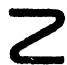
\includegraphics[keepaspectratio]{images/part001_1db83a62.jpg}}

Remark. If X is locally compact but not compact, then a closed equivalence relation R on X need not be Hausdorff (Chapter IX, § 4, Exercise 14); and even if R is Hausdorff, X/R need not be locally compact (Exercise 17). However, we have the following criterion:

PROPOSITION 10. Let X be a locally compact space, R an open Hausdorff equivalence relation on X, and let \(f: \mathrm{X} \to \mathrm{X}/\mathrm{R}\) be the canonical mapping. Then \(\mathrm{X}/\mathrm{R}\) is locally compact, and if \(\mathbf{K}'\) is any compact subset of \(\mathrm{X}/\mathrm{R}\) there is a compact subset K of X such that \(f(\mathbf{K}) = \mathbf{K}'\) .

The first assertion is a consequence of the facts that each \(x \in \mathbf{X}\) has a compact neighbourhood \(\mathbf{V}\) and that \(f(\mathbf{V})\) is a compact neighbourhood of \(f(x)\) ( \(\S 5, \text{no. } 3, \text{ Proposition } 5\) and \(\S 9, \text{ no. } 4, \text{ Theorem } 2, \text{ Corollary } 1\) ). For each \(y \in \mathbf{K}'\) let \(\mathbf{V}(y)\) be a compact neighbourhood of some point of \(\overline{f}^1(y)\) in \(\mathbf{X}\) , so that \(f(\mathbf{V}(y))\) is a compact neighbourhood of \(y\) . There are a finite number of points \(y_i \in \mathbf{K}'\) such that the \(f(\mathbf{V}(y_i))\) cover \(\mathbf{K}'\) . Let \(\mathbf{K}_1\) be the compact set \(\bigcup_i \mathbf{V}(y_i)\) in \(\mathbf{X}\) ; we have \(\mathbf{K}' \subset f(\mathbf{K}_1)\) ; hence \(\mathbf{K} = \mathbf{K}_1 \cap \overline{f}^1(\mathbf{K}')\) is compact (because it is closed in \(\mathbf{K}_1\) ) and \(f(\mathbf{K}) = \mathbf{K}'\) .

\section{CONNECTEDNESS}
